\documentclass[11pt]{amsart}
\usepackage[margin=1.15in]{geometry}
\usepackage{amsmath,amssymb,amsthm}
\usepackage{enumitem}
\usepackage{tikz}
\usepackage[hidelinks]{hyperref}

\newtheorem{theorem}{Theorem}[section]
\newtheorem{lemma}[theorem]{Lemma}
\newtheorem{proposition}[theorem]{Proposition}
\newtheorem{corollary}[theorem]{Corollary}
\newtheorem{conjecture}[theorem]{Conjecture}
\theoremstyle{definition}
\newtheorem{definition}[theorem]{Definition}
\newtheorem{setup}[theorem]{Setup}
\theoremstyle{remark}
\newtheorem{remark}[theorem]{Remark}
\numberwithin{equation}{section}
\raggedbottom

\newcommand{\cl}{\operatorname{cl}}
\newcommand{\si}{\operatorname{si}}
\newcommand{\lam}{\lambda}
\newcommand{\GW}{\mathsf{G}}
\newcommand{\FA}{\mathsf{A}}
\newcommand{\FB}{\mathsf{B}}

\begin{document}

\title[Sharp size bounds for $3$-connected positroids]{Sharp size bounds for $3$-connected positroids without a long line minor}
\author{Knowledge Sense}
\address{Knowledge Sense}
\email{math@knowledgesense.jp}
\date{8 October 2026}
\subjclass[2020]{Primary 05B35; Secondary 05E14}
\keywords{Positroid, extremal matroid theory, excluded minor, $3$-connected matroid, generalized whirl}

\begin{abstract}
We prove that every $3$-connected positroid of rank $r\ge2$ with no $U_{2,\ell+2}$-minor has at most $r(\ell+1)/2$ elements if $\ell\ge3$ is odd, and at most $r\ell/2+1$ elements if $\ell\ge4$ is even. This is the parity-sensitive bound conjectured by Boretsky and Walsh, and it is sharp for every rank: for $r\ge3$ it is attained by generalized whirls when $\ell$ is odd and by generalized whirls with one additional point when $\ell$ is even, and for $r=2$ by $U_{2,\ell+1}$. For $\ell\ge4$ we determine all matroids attaining the bound. When $\ell$ is odd they are the generalized whirls. When $\ell$ is even they are obtained from a path of lines, whose junction points form a matroid with exactly one circuit, by freely adding points on the lines; for $\ell=4$ only, a second family, built from three paths of triangles, also occurs. The bound is proved by induction on the rank, using a contraction that preserves $3$-connectivity and loses few elements; the classification reconstructs an extremal matroid from a smaller one, using nonseparating lines and the cyclic order of a positroid.
\end{abstract}

\maketitle

\section{Introduction}

A \emph{positroid} is a matroid that can be represented by a real matrix all of whose maximal minors are nonnegative. Positroids were introduced by Postnikov~\cite{Pos06} in the study of the totally nonnegative Grassmannian, and they admit several combinatorial descriptions~\cite{ARW16,Pos06}. They form a minor-closed class that is closed under duality~\cite{ARW16}, and Bonin~\cite{Bon24} characterized them by a cyclic interval property of their connected flats.

Given a class $\mathcal M$ of matroids, extremal matroid theory asks for the largest number of elements of a simple rank-$r$ matroid in $\mathcal M$, together with the matroids that attain it~\cite{Kun93}. A natural setting is the exclusion of a long line: Kung~\cite{Kun93} bounded the size of simple rank-$r$ matroids with no $U_{2,\ell+2}$-minor, Geelen and Nelson~\cite{GN10} determined the exact maximum for large rank, and Geelen, Nelson and Walsh~\cite{GNW24} did the same for complex-representable matroids. Boretsky and Walsh~\cite{BW25,BW26} began the study of positroids in this context. They proved that a simple rank-$r$ positroid with no $U_{2,\ell+2}$-minor has at most $\ell(r-1)+1$ elements, with equality exactly for parallel connections of copies of $U_{2,\ell+1}$. Chen and Li~\cite[Theorem~1.1 and Corollary~1.2]{CL26} recently proved the same bound for gammoids, and hence for transversal matroids. The extremal positroids in these results are not $3$-connected when $r\ge 3$, which raises the question of the maximum size of a $3$-connected positroid without a long line minor~\cite[Section~6.1]{BW25}, \cite[Section~7.1]{BW26v2}. For comparison, Quail~\cite[Theorem~3.8 and Proposition~3.12]{Qua24} described the ternary positroids, a class that excludes both $U_{2,5}$ and $U_{3,5}$, and characterized the quaternary positroids as those excluding $U_{2,6}$, $U_{4,6}$ and $P_6$; these results concern classes defined by more than one excluded minor.

Generalized whirls are classical. De Mier~\cite[Section~7.1.2, pp.~76--77]{dM03} defined, for $n,s\ge3$, the $(n,s)$-whirl: a rank-$n$ matroid with $n(s-1)$ elements whose $n$ long lines have $s$ elements each, obtained from the rank-$n$ whirl by freely adding points on its lines. For $r\ge3$ and $\ell\ge3$, Boretsky and Walsh~\cite[Section~6.1]{BW25} considered the matroid $W(r,\ell)$ obtained from a basis $b_1,\dots,b_r$ by freely placing $\lfloor(\ell-1)/2\rfloor$ elements on each line spanned by $b_i,b_{i+1}$ (indices modulo $r$), and the matroid $W(r,\ell)^+$ obtained from it by freely placing one further element on the line spanned by $b_1,b_2$. They observed that $W(r,\ell)$ and $W(r,\ell)^+$ are $3$-connected positroids, that $W(r,\ell)$ has no $U_{2,\ell+2}$-minor, and that $W(r,\ell)^+$ has none when $\ell$ is even. Their convention for $r=2$ differs from the one used below. Throughout the paper we write
\[
t=\Big\lfloor\frac{\ell+1}{2}\Big\rfloor,\qquad \varepsilon=\ell+1-2t\in\{0,1\},
\]
so that $\ell=2t-1$ when $\ell$ is odd and $\ell=2t$ when $\ell$ is even. Our first result is the following bound.

\begin{theorem}\label{thm:bound}
Let $r\ge 2$ and $\ell\ge 3$ be integers. Every $3$-connected positroid of rank $r$ with no $U_{2,\ell+2}$-minor has at most $tr+\varepsilon$ elements. Equivalently, it has at most $r(\ell+1)/2$ elements if $\ell$ is odd and at most $r\ell/2+1$ elements if $\ell$ is even. The bound is attained for all $r\ge 2$ and $\ell\ge 3$.
\end{theorem}

\emph{Relation to the conjectures of Boretsky and Walsh.} For $r\ge3$ we have $|W(r,\ell)|=r+r\lfloor(\ell-1)/2\rfloor=tr$. Hence the bound of Theorem~\ref{thm:bound} is attained by $W(r,\ell)$ when $\ell$ is odd and by $W(r,\ell)^+$ when $\ell$ is even, and for $r=2$ it is attained by $U_{2,\ell+1}$. In the first arXiv version of their paper~\cite[Conjecture~6.1]{BW25} and in their FPSAC 2026 extended abstract~\cite[Conjecture~6.1]{BW26a}, Boretsky and Walsh conjectured the bound $r+r\lfloor(\ell-1)/2\rfloor$ for odd $\ell$ and $r+r\lfloor(\ell-1)/2\rfloor+1$ for even $\ell$; this is $tr+\varepsilon$, so Theorem~\ref{thm:bound} proves that conjecture. In the second arXiv version~\cite[Conjecture~7.1]{BW26v2}, the conjectured bound is $r(\lfloor\ell/2\rfloor+1)$. It equals $tr$ for odd $\ell$ and exceeds $tr+1$ by $r-1$ for even $\ell$, so it also follows from Theorem~\ref{thm:bound}. In the present paper, $W(r,\ell)$ and $W(r,\ell)^+$ reappear as the generalized whirls $\GW_r(t)$ and as the heavy members of Family~$\FA$ below, and we include proofs of the properties we use. The bound $\ell(r-1)+1$ of~\cite{BW26,CL26} concerns simple matroids without a connectivity hypothesis and has a different extremal family.

Our second result determines the extremal matroids for $\ell\ge4$. We summarize the three families here; precise definitions are given in Section~\ref{sec:families}, and Figure~\ref{fig:models} shows them schematically. A point is \emph{freely added} on a line if it is added by the principal extension on that line (Section~\ref{sec:free}).
\begin{itemize}[leftmargin=2em]
\item For $r\ge3$ and $t\ge2$, the generalized whirl $\GW_r(t)$ is obtained from a basis $v_1,\dots,v_r$ by freely adding $t-1$ points on each line spanned by $v_i,v_{i+1}$, indices modulo $r$. Thus $\GW_r(t)=W(r,2t-1)=W(r,2t)$ for $r\ge3$, and $\GW_r(t)$ corresponds to the $(r,t+1)$-whirl of~\cite{dM03}. We also put $\GW_2(t)=U_{2,2t}$.
\item For $r\ge2$ and $t\ge2$, Family $\FA$ consists of the matroids $\FA_r(C;t)$ defined as follows. Let $v_0,\dots,v_r$ be junctions and let $C\subseteq\{v_0,\dots,v_r\}$ satisfy $|C|\ge3$ and $v_0,v_r\in C$. The matroid on the junctions has $C$ as its only circuit, every junction outside $C$ being a coloop, and $\FA_r(C;t)$ is obtained by freely adding $t-1$ points on each line spanned by $v_i,v_{i+1}$ with $0\le i\le r-1$. For $r\ge3$ the matroid $W(r,2t)^+$ is isomorphic to a member of this family.
\item For positive integers $a,b,c$, the matroid $\FB(a,b,c)$ is built on three disjoint paths of $a$, $b$ and $c$ triangles. The dual of the matroid on the junctions of these triangles has rank two; in it the junctions lying on two triangles are loops, and the six ends of the paths form three parallel pairs, each joining ends of two different paths. The matroid $\FB(a,b,c)$ has rank $a+b+c+1$ and occurs only for $t=2$.
\end{itemize}

\begin{theorem}\label{thm:classification}
Let $r\ge 2$ and $\ell\ge 4$ be integers, and let $M$ be a $3$-connected positroid of rank $r$. Then $M$ has no $U_{2,\ell+2}$-minor and has exactly $tr+\varepsilon$ elements if and only if $M$ is isomorphic to one of the following matroids:
\begin{enumerate}[label=\textup{(\roman*)}]
\item $\GW_r(t)$, if $\ell=2t-1$ is odd;
\item $\FA_r(C;t)$ for some $C\subseteq\{v_0,\dots,v_r\}$ with $|C|\ge3$ and $v_0,v_r\in C$ \textup{(}Definition~\textup{\ref{def:families}(b))}, if $\ell=2t$ is even;
\item $\FB(a,b,c)$ for some positive integers $a,b,c$ with $a+b+c=r-1$, if $\ell=4$.
\end{enumerate}
\end{theorem}

Different parameters in (ii) and (iii) may give isomorphic matroids; we do not determine when this happens. The matroids $\FB(a,b,c)$ have rank at least four, and for $\ell=4$ they differ from all members of Family~$\FA$: a matroid in Family~$\FA$ of rank $r\ge3$ has $r$ nonseparating long lines, whereas $\FB(a,b,c)$ has $r-1$. The hypothesis $\ell\ge4$ in Theorem~\ref{thm:classification} is used in the proof: Lemma~\ref{lem:equality}(a) applies Theorem~\ref{thm:bound} with $\ell-1$ in place of $\ell$, which requires $\ell-1\ge3$.

\emph{Outline of the proofs.} In Section~\ref{sec:prelim} we collect the matroid and positroid facts we need; the main tools are Bonin's cyclic interval characterization of positroids and the principal extension. In Section~\ref{sec:interiors} we show that an interior point of a nonseparating long line of a positroid is freely placed on it, and that contracting such a point preserves $3$-connectivity. Combined with Wu's theorem on vertically contractible elements and Tutte's linking theorem, this yields in Section~\ref{sec:bound} an element whose contraction is $3$-connected and loses at most $\lfloor q/2\rfloor$ points, where $U_{2,q}$ is the longest uniform line minor; Theorem~\ref{thm:bound} follows by induction on the rank. Section~\ref{sec:families} establishes the properties of the three families, which gives the sufficiency part of Theorem~\ref{thm:classification}. The necessity part occupies Sections~\ref{sec:equality}--\ref{sec:four}: we contract an interior point $e$ of a nonseparating line $L$ of an extremal matroid $M$, identify the smaller extremal matroid $N$ by induction, and reconstruct $M$ from $N$. The reconstruction depends on the position of the collapsed point $p$ of $L$ in $N$. Contracting further lines of $N$ that avoid $p$, simultaneously in $M$ and in $N$, reduces the problem to rank three, where all extremal matroids are known explicitly; a skewness argument transports collinearities from rank three back to $M$. Section~\ref{sec:odd} treats odd $\ell$, Section~\ref{sec:even} treats even $\ell\ge6$, and Section~\ref{sec:four} treats $\ell=4$, where the second family $\FB$ appears.

\emph{Dependencies.} Besides standard matroid theory~\cite{Oxl11}, the proofs use the following published results, which we do not reprove: the closure properties of positroids under minors, duality and noncrossing direct sums~\cite{ARW16}; Bonin's characterization of positroid orders and its corollary on connected flats~\cite[Theorem~3.2(4) and Corollary~3.4]{Bon24}; the fact that $M(K_4)$ is not a positroid~\cite[Section~3]{Bon24}; the fact that every $3$-connected binary matroid with at least four elements has an $M(K_4)$-minor~\cite[Corollary~12.2.13]{Oxl11}; Wu's theorem on minimally $3$-connected matroids, in the form stated in~\cite[Theorem~12.6]{Oxl96}; and Tutte's linking theorem in the form that preserves the two restrictions~\cite[Theorem~8.5.7]{Oxl11}. No computer calculation is used.

\section{Preliminaries}\label{sec:prelim}

\subsection{Matroids}
We follow Oxley~\cite{Oxl11}. All matroids are finite. For a matroid $M$ we write $E(M)$ for its ground set, $r_M$ or $r$ for its rank function, $r(M)=r_M(E(M))$, and $\cl_M$ for its closure operator. For $X\subseteq E(M)$ the \emph{connectivity function} is
\[
\lam_M(X)=r_M(X)+r_M(E(M)-X)-r(M).
\]
For $k\in\{1,2\}$, a \emph{$k$-separation} of $M$ is a partition $(X,Y)$ of $E(M)$ with $|X|,|Y|\ge k$ and $\lam_M(X)<k$. A matroid is \emph{connected} if its ground set is nonempty and it has no $1$-separation. We call $M$ \emph{$3$-connected} if $|E(M)|\ge4$ and $M$ has no $1$- or $2$-separation. A $3$-connected matroid in this sense is simple and has no coloops. The convention $|E(M)|\ge4$ excludes only matroids with at most three elements, and since $tr+\varepsilon\ge 2t\ge4$, it does not affect Theorems~\ref{thm:bound} and~\ref{thm:classification}.

A \emph{line} is a flat of rank two, and a line is \emph{long} if it has at least three elements. A \emph{triangle} is a three-element circuit. A long line $L$ of $M$ is \emph{nonseparating} if $L\ne E(M)$ and $M/L$ is connected. For a matroid $M$ with $r(M)\ge2$ we let $q(M)$ be the largest integer $q$ such that $M$ has a $U_{2,q}$-minor; if $M$ is simple then $q(M)\ge2$. For a simple matroid $M$ with $r(M)\ge2$ and $x\in E(M)$, the parallel classes of $M/x$ are the sets $K-x$ for the lines $K$ of $M$ through $x$, and $M/x$ is loopless. Hence the \emph{loss}
\begin{equation}\label{eq:loss}
\delta_M(x)=|E(M)|-|E(\si(M/x))|=1+\sum_{K}(|K|-2),
\end{equation}
where the sum is over the long lines $K$ of $M$ containing $x$.

We use the rank formulas $r_{M/X}(Y)=r_M(X\cup Y)-r_M(X)$ and $r_{M^*}(Y)=|Y|+r_M(E(M)-Y)-r(M)$. Two sets $X,Y$ are \emph{skew} if $r_M(X\cup Y)=r_M(X)+r_M(Y)$. If $C$ is skew to a set $F$ and $C\cap F=\emptyset$, then submodularity gives $r_M(X\cup C)=r_M(X)+r_M(C)$ for every $X\subseteq F$, so $r_{M/C}(X)=r_M(X)$ for every $X\subseteq F$.

\begin{lemma}\label{lem:basic}
Let $M$ be a matroid.
\begin{enumerate}[label=\textup{(\alph*)}]
\item If $M'$ is obtained from a connected matroid $M$ by adding elements each parallel to an element of $M$, then $M'$ is connected.
\item A loopless matroid of rank one is connected, and a loopless matroid of rank two with at least three parallel classes is connected.
\item If $M$ is $3$-connected and $x\in E(M)$, then $M/x$ is connected.
\item If $X\subseteq E(M)$ is connected in $M$, that is $M|X$ is connected, and $y$ is a nonloop of $M$ in $\cl_M(X)$, then $X\cup\{y\}$ lies in a single component of $M$.
\end{enumerate}
\end{lemma}

\begin{proof}
Parts (a), (b) and (d) are standard: two parallel nonloops form a circuit, elements in a common circuit lie in a common component, and in (b) any two nonparallel elements lie in a triangle together with a third element. For (c), suppose that $M/x=N_1\oplus N_2$ with $E(N_1)$ and $E(N_2)$ nonempty. Then
\[
\lam_M(E(N_1))\le \big(r_{M/x}(E(N_1))+1\big)+\big(r_{M/x}(E(N_2))+1\big)-\big(r(M/x)+1\big)=1.
\]
Since $M$ is $3$-connected, one side, say $E(N_1)=\{y\}$, has one element. Then $y$ is a loop or a coloop of $M/x$. In the first case $\{x,y\}$ is a parallel pair of $M$; in the second case $r_M(E(M)-y)=r(M)-1$ and $y$ is a coloop of $M$. Both contradict $3$-connectivity.
\end{proof}

\begin{lemma}\label{lem:qrec}
Let $M$ be a simple matroid.
\begin{enumerate}[label=\textup{(\alph*)}]
\item Every simple minor of a matroid $P$ is a minor of $\si(P)$.
\item If $r(M)=2$ then $q(M)=|E(M)|$. If $r(M)\ge3$ then $q(M)=\max_{x\in E(M)}q(\si(M/x))$.
\end{enumerate}
\end{lemma}

\begin{proof}
(a) Write a simple minor as $P/C\backslash D$ with $C$ independent. Its elements are pairwise nonparallel nonloops of $P$, since contraction preserves parallelism and loops. Replacing an element of $C$ by a parallel element does not change the minor on the remaining elements. Hence the minor is a minor of $\si(P)$ for a suitable choice of representatives.

(b) The first assertion holds because $M$ is uniform. Let $r(M)\ge3$ and let $U$ be a $U_{2,m}$-minor of $M$ with ground set $T$. Write $U=(M/C)|T$; we may assume that $C$ is independent, since replacing $C$ by a basis $C_0$ of $C$ only turns the elements of $C-C_0$ into loops of $M/C_0$, which are deleted. While $T\cup C$ does not span $M$, add to $C$ an element $y\notin\cl_M(T\cup C)$. Then $C\cup y$ is independent, and for $X\subseteq T$ we have $r_M(X\cup C\cup y)=r_M(X\cup C)+1$ and $r_M(C\cup y)=r_M(C)+1$, so $r_{M/(C\cup y)}(X)=r_{M/C}(X)$ and still $U=(M/(C\cup y))|T$. When the procedure stops, $C$ is independent, $T\cup C$ spans $M$ and $r(M)=r_{M/C}(T)+|C|=2+|C|$. Thus
\begin{equation}\label{eq:standardC}
U=(M/C)|T\quad\text{with $C$ independent, $C\cap T=\emptyset$ and $|C|=r(M)-2$.}
\end{equation}
As $|C|\ge1$, $U$ is a minor of $M/x$ for any $x\in C$ and, by (a), of $\si(M/x)$. The reverse inequality is clear.
\end{proof}

\subsection{Positroids and cyclic intervals}\label{sec:positroids}
A \emph{positroid order} of a matroid $M$ is a linear order $<$ on $E(M)$ such that $M$ is represented by a real matrix whose columns are ordered by $<$ and whose maximal minors are nonnegative. A matroid is a positroid if it has a positroid order. By~\cite[Lemma~3.3]{ARW16}, every cyclic shift of a positroid order is a positroid order, so we regard a positroid order as a \emph{cyclic} order. For a cyclic order on a set $E$, a \emph{cyclic interval} is a set of consecutive elements. If $I$ is a cyclic interval with $2\le|I|<|E|$, its two \emph{endpoints} are its first and last elements and its other elements are \emph{interior} points of $I$.

\begin{proposition}[\cite{ARW16,Bon24}]\label{prop:positroid}
Let $M$ be a positroid with a positroid order $<$.
\begin{enumerate}[label=\textup{(P\arabic*)}]
\item For $X\subseteq E(M)$, the restriction of $<$ to $E(M)-X$ is a positroid order of $M\backslash X$ and of $M/X$, and $<$ is a positroid order of $M^*$ \textup{\cite[Proposition~3.5]{ARW16}}.
\item If $S_1,\dots,S_k$ is a noncrossing partition of a cyclically ordered set $E$ and $M_i$ is a positroid on $S_i$ with the induced order, then $M_1\oplus\dots\oplus M_k$ is a positroid with the order of $E$ \textup{\cite[Theorem~7.6]{ARW16}}.
\item Suppose that $M$ is loopless. A linear order on $E(M)$ is a positroid order if and only if, for every proper flat $F$ of $M$ with $|F|\ge2$ and $M|F$ connected and every component $K$ of $M/F$ with $|K|\ge2$, the set $K$ is contained in a cyclic interval disjoint from $F$ \textup{\cite[Theorem~3.2, (1)$\Leftrightarrow$(4)]{Bon24}}.
\item If $M$ is loopless and $F$ is a flat such that $M|F$ and $M/F$ are connected, then $F$ is a cyclic interval of every positroid order \textup{\cite[Corollary~3.4]{Bon24}}.
\item $M(K_4)$ is not a positroid \textup{\cite[Section~3, after Corollary~3.4]{Bon24}}.
\end{enumerate}
\end{proposition}

Every uniform matroid is a positroid in every order, as it is represented by a matrix whose maximal minors are all positive (for instance a Vandermonde matrix with increasing positive nodes). By (P1) and (P5), a positroid has no minor isomorphic to $M(K_4)$. By (P4), every nonseparating long line of a simple positroid is a cyclic interval of every positroid order, and so is every parallel class of a loopless positroid of rank two, since such a class is a flat whose restriction and contraction are connected.

Whenever we pass to a minor of a positroid with a fixed positroid order, we use the induced order, which is a positroid order by (P1). In particular simplification uses the induced order on the retained representatives. We shall use the following elementary facts about a cyclic order on a set $E$ with $|E|\ge3$; each element $x$ has two distinct \emph{neighbours}, the elements immediately before and after it.

\begin{lemma}\label{lem:intervals}
Let $E$ be cyclically ordered with $|E|\ge3$, and let $I,I'$ be cyclic intervals with at least two elements.
\begin{enumerate}[label=\textup{(\alph*)}]
\item If $x\in I$, then $I$ contains a neighbour of $x$; if $x$ is an interior point of $I$, then $I$ contains both neighbours of $x$.
\item If $I\cap I'=\{x\}$, then $x$ is an endpoint of both $I$ and $I'$.
\item No element lies in three cyclic intervals of size at least two any two of which meet only in that element.
\item A cyclic interval containing distinct elements $x,y$ contains one of the two arcs of $E$ from $x$ to $y$.
\end{enumerate}
\end{lemma}

\begin{proof}
Parts (a) and (d) are immediate from the definitions. For (b), if $x$ were interior to $I$, then $I$ would contain both neighbours of $x$ and $I'$ would contain one of them by (a). Part (c) follows from (a), since the three intervals would contain three neighbours of $x$ that are pairwise distinct, while $x$ has only two.
\end{proof}

Applied to nonseparating long lines of a simple positroid, Lemma~\ref{lem:intervals} shows that two such lines meet in at most one point, which is then an endpoint of both, that no point lies on three of them, and that an interior point of one of them lies on no other.

\subsection{Free points}\label{sec:free}
Let $a,b$ be independent elements of a matroid $M$ and let $f\in E(M)-\{a,b\}$. We say that $f$ is \emph{freely placed on $\{a,b\}$} if $f\in\cl_M(\{a,b\})$ and, for every $X\subseteq E(M)-f$,
\[
f\in\cl_M(X)\ \Longrightarrow\ \{a,b\}\subseteq\cl_M(X).
\]
The converse implication always holds. If $K$ is a line containing $f$ and at least two other elements, we say that $f$ is \emph{freely placed on $K$} if it is freely placed on some, equivalently every, independent pair of elements of $K-f$; equivalently, $f\in\cl_M(X)$ implies $K\subseteq\cl_M(X)$ for $X\subseteq E(M)-f$. Given independent $a,b$ in a matroid $M$ and a new element $f$, the \emph{principal extension} $M+_{ab}f$ is the extension of $M$ in which $f\in\cl(X)$ if and only if $\{a,b\}\subseteq\cl_M(X)$, for $X\subseteq E(M)$; it exists and is the extension corresponding to the modular cut of flats containing $\{a,b\}$~\cite[Section~7.2]{Oxl11}. In $M+_{ab}f$ the element $f$ is freely placed on $\{a,b\}$. We also say that $f$ is \emph{freely added} on the line spanned by $a,b$.

\begin{lemma}\label{lem:free}
Let $f$ be freely placed on an independent pair $\{a,b\}$ in a matroid $M$, and let $g\in E(M)-\{a,b,f\}$.
\begin{enumerate}[label=\textup{(\alph*)}]
\item $f$ is freely placed on $\{a,b\}$ in $M\backslash g$.
\item If $\{a,b\}$ is independent in $M/g$, then $f$ is freely placed on $\{a,b\}$ in $M/g$.
\item If $c,d\in E(M)-f$ are independent and $M'=M+_{cd}g'$ for a new element $g'$, then $f$ is freely placed on $\{a,b\}$ in $M'$.
\item If $M$ is simple, then every triangle of $M$ containing $f$ lies in the line $\cl_M(\{a,b\})$.
\end{enumerate}
\end{lemma}

\begin{proof}
Part (a) holds because closures in $M\backslash g$ are traces of closures in $M$. For (b), if $f\in\cl_{M/g}(X)$ then $f\in\cl_M(X\cup g)$, so $\{a,b\}\subseteq\cl_M(X\cup g)$ and $\{a,b\}\subseteq\cl_{M/g}(X)$; also $f\in\cl_{M/g}(\{a,b\})$. For (d), if $\{f,x,y\}$ is a triangle then $\{a,b\}\subseteq\cl_M(\{x,y\})$, and as both $\cl_M(\{x,y\})$ and $\cl_M(\{a,b\})$ are lines, they are equal.

For (c), let $X\subseteq E(M')-f$ with $f\in\cl_{M'}(X)$. If $g'\notin X$, then $f\in\cl_M(X)$ and we are done. Let $X=X_0\cup g'$. If $g'\in\cl_{M'}(X_0)$ or $f\in\cl_{M'}(X_0)$, then $f\in\cl_M(X_0)$ and again $\{a,b\}\subseteq\cl_M(X_0)$. Otherwise the exchange property gives $g'\in\cl_{M'}(X_0\cup f)$, so $\{c,d\}\subseteq\cl_M(X_0\cup f)$ by the definition of $M'$. Since $g'\notin\cl_{M'}(X_0)$, not both of $c,d$ lie in $\cl_M(X_0)$, hence $r_M(X_0\cup\{c,d\})=r_M(X_0)+1=r_M(X_0\cup f)$ and $\cl_M(X_0\cup\{c,d\})=\cl_M(X_0\cup f)$. As $g'\in\cl_{M'}(X_0\cup\{c,d\})$ and $r_{M'}(X_0\cup g')=r_M(X_0)+1$, we get $\cl_{M'}(X_0\cup g')=\cl_{M'}(X_0\cup\{c,d\})\ni f$, so $f\in\cl_M(X_0\cup\{c,d\})$. Freeness of $f$ in $M$ gives $\{a,b\}\subseteq\cl_M(X_0\cup\{c,d\})\subseteq\cl_{M'}(X_0\cup g')$.
\end{proof}

\begin{definition}\label{def:freemodel}
Let $K$ be a matroid and let $(f_1,P_1),\dots,(f_m,P_m)$ be pairs in which the $f_j$ are distinct new elements and each $P_j$ is an independent pair of elements of $K$. The \emph{free extension} of $K$ by these pairs is the matroid obtained from $K$ by successively forming principal extensions $+_{P_1}f_1,\dots,+_{P_m}f_m$, where each $P_j$ is regarded as a pair of elements of the current matroid. We call $K$ its \emph{core}.
\end{definition}

\begin{lemma}\label{lem:unique}
Let $K$ and $(f_j,P_j)_{j\le m}$ be as in Definition~\ref{def:freemodel}, and let $M$ be their free extension.
\begin{enumerate}[label=\textup{(\alph*)}]
\item Each $f_j$ is freely placed on $P_j$ in $M$.
\item If $M'$ is a matroid on $E(K)\cup\{f_1,\dots,f_m\}$ with $M'|E(K)=K$ in which each $f_j$ is freely placed on $P_j$, then $M'=M$. In particular $M$ does not depend on the order of the pairs.
\end{enumerate}
\end{lemma}

\begin{proof}
Part (a) follows from Lemma~\ref{lem:free}(c) by induction on $m$. For (b) we induct on $m$, the case $m=0$ being trivial. By Lemma~\ref{lem:free}(a), the matroids $M'\backslash f_m$ and $M\backslash f_m$ satisfy the hypotheses for the first $m-1$ pairs, so they are equal by induction. In both $M'$ and $M$, a flat $F$ of this common deletion spans $f_m$ if and only if $P_m\subseteq F$. A single-element extension is determined by the set of flats that span the new element~\cite[Section~7.2]{Oxl11}, so $M'=M$.
\end{proof}

\begin{lemma}\label{lem:triangles}
Let $M$ be a free extension of a core $K$ by pairs $(f_j,P_j)$, and assume that $M$ is simple. For every line $X$ of $K$,
\[
\cl_M(X)=X\cup\{f_i:\ P_i\subseteq X\},
\]
and every long line of $M$ is of this form for a line $X$ of $K$ that is either long in $K$ or equal to $\cl_K(P_j)$ for some $j$.
\end{lemma}

\begin{proof}
For $Y\subseteq E(K)$ we have $\cl_M(Y)\cap E(K)=\cl_K(Y)$, and by Lemma~\ref{lem:unique}(a) we have $f_i\in\cl_M(Y)$ if and only if $P_i\subseteq\cl_K(Y)$. This gives the displayed formula. A long line of $M$ containing some $f_i$ contains a triangle through $f_i$, hence equals $\cl_M(P_i)=\cl_M(\cl_K(P_i))$ by Lemma~\ref{lem:free}(d). A long line of $M$ containing no $f_i$ is a flat of $M$ contained in $E(K)$, hence a long line $X$ of $K$ with $\cl_M(X)=X$.
\end{proof}

\section{Interior points and contractions}\label{sec:interiors}

\begin{lemma}\label{lem:delete4}
Let $P$ be a $3$-connected matroid of rank at least three and let $S$ be a line of $P$ with $|S|\ge4$. Then $P\backslash x$ is $3$-connected for every $x\in S$.
\end{lemma}

\begin{proof}
Since $P$ has no coloops, $r(P\backslash x)=r(P)$, and $|E(P)|\ge|S|+1\ge5$. Let $(A,B)$ be a partition of $E(P)-x$. As $|S-x|\ge3$, one side, say $B$, contains two elements of $S-x$ and therefore spans $x$. Hence $\lam_{P\backslash x}(A)=r(A)+r(B\cup x)-r(P)=\lam_P(A)$, and a $1$- or $2$-separation $(A,B)$ of $P\backslash x$ would give the separation $(A,B\cup x)$ of $P$ of the same order.
\end{proof}

\begin{lemma}\label{lem:spanning}
Let $R$ be a simple matroid with a $3$-connected restriction $Q$ such that $E(Q)$ spans $R$. Then $R$ is $3$-connected. Consequently, if $N$ is a restriction of a simple matroid $M$ with $r(N)=r(M)$, $e\in E(N)$, and $\si(N/e)$ is $3$-connected, then $\si(M/e)$ is $3$-connected.
\end{lemma}

\begin{proof}
Let $(A,B)$ be a partition of $E(R)$ with $A,B\ne\emptyset$. If both $A$ and $B$ contain at least two elements of $E(Q)$, then $\lam_R(A)\ge\lam_Q(A\cap E(Q))\ge2$ because $r(R)=r(Q)$. Otherwise one side, say $A$, contains at most one element of $E(Q)$; as $Q$ has no coloops, $B\cap E(Q)$ spans $Q$ and hence $R$, so $\lam_R(A)=r_R(A)$, which is at least $1$ and is at least $2$ when $|A|\ge2$, by simplicity. Thus $R$ has no $1$- or $2$-separation, and $|E(R)|\ge|E(Q)|\ge4$.

For the second statement, distinct parallel classes of $N/e$ lie in distinct parallel classes of $M/e$, and loops of $N/e$ are loops of $M/e$. Hence we can choose $\si(M/e)$ so that it contains $\si(N/e)$ as a restriction, which spans because $N$ spans $M$. The first statement applies.
\end{proof}

Following~\cite[p.~163]{Oxl96}, a matroid $P$ with $r(P)\ge3$ is \emph{vertically $3$-connected} if there is no partition $(X,Y)$ of $E(P)$ with $\min\{r(X),r(Y)\}\ge k$ and $\lam_P(X)\le k-1$ for some $k\in\{1,2\}$. An element $x$ of a $3$-connected matroid $P$ is \emph{vertically contractible} if $P/x$ is vertically $3$-connected. A $3$-connected matroid is \emph{minimally $3$-connected} if no single-element deletion is $3$-connected.

\begin{theorem}[{Wu~\cite{Wu98}; see~\cite[Theorem~12.6]{Oxl96}}]\label{thm:wu}
A minimally $3$-connected matroid with at least four elements has at least three vertically contractible elements, and it has exactly three if and only if it is isomorphic to $M^*(K'''_{3,k})$ for some $k\ge2$.
\end{theorem}

We use only that the matroids $M^*(K'''_{3,k})$ are cographic and hence binary.

\begin{lemma}\label{lem:vertical}
Let $P$ be a simple matroid with $r(P)\ge4$ and let $x\in E(P)$. If $P/x$ is vertically $3$-connected, then $\si(P/x)$ is $3$-connected.
\end{lemma}

\begin{proof}
Put $Q=\si(P/x)$; it is simple of rank at least three. If $(X,Y)$ were a $k$-separation of $Q$ with $k\in\{1,2\}$, then adding the parallel copies to the sides containing their representatives would give a partition of $E(P/x)$, which is loopless, with the same ranks; as $|X|\ge k$ and $Q$ is simple, $r(X),r(Y)\ge k$, and this would be a vertical $k$-separation. Finally $|E(Q)|\ge4$, since a simple matroid of rank at least three on three elements is free and has a $1$-separation with sides of rank at least one.
\end{proof}

\begin{lemma}\label{lem:wu}
Let $M$ be a $3$-connected positroid with $r(M)\ge4$ and let $L$ be a line of $M$. There is an element $e\notin L$ such that $\si(M/e)$ is $3$-connected.
\end{lemma}

\begin{proof}
Starting from $M$, delete one element at a time as long as the resulting matroid is $3$-connected, and let $N$ be the matroid obtained when no such deletion is possible. Each deletion preserves the rank, so $r(N)=r(M)\ge4$, and $N$ is a minimally $3$-connected positroid. By Lemma~\ref{lem:delete4}, $N$ has no line with four or more elements, so $|E(N)\cap L|\le3$. The matroid $N$ is not binary: a $3$-connected binary matroid with at least four elements has an $M(K_4)$-minor~\cite[Corollary~12.2.13]{Oxl11}, while $N$ has none by Proposition~\ref{prop:positroid}. By Theorem~\ref{thm:wu}, $N$ has at least four vertically contractible elements, so one of them, $e$, lies outside $L$. By Lemma~\ref{lem:vertical}, $\si(N/e)$ is $3$-connected, and by Lemma~\ref{lem:spanning}, so is $\si(M/e)$.
\end{proof}

\begin{lemma}[Interior points are free]\label{lem:interiorfree}
Let $M$ be a simple positroid with a positroid order, and let $L$ be a long line of $M$ that is a cyclic interval. Then every interior point $e$ of $L$ is freely placed on $L$.
\end{lemma}

\begin{proof}
Let $X\subseteq E(M)-e$ with $e\in\cl(X)$. If $X$ contains a point of $L-e$, then this point and $e$ span $L$, so $L\subseteq\cl(X)$. Suppose that $X\cap L=\emptyset$ and $L\not\subseteq\cl(X)$. Choose a circuit $C\subseteq X\cup e$ with $e\in C$, and put $F=\cl(C)$. Then $F\subseteq\cl(X)$, so $F$ contains no point of $L-e$ (two points of $L$ in $F$ would give $L\subseteq F$), and $F\cap L=\{e\}$; in particular $F$ is a proper flat. By simplicity $|C|\ge3$. The restriction $M|F$ is connected: $C$ is connected, and every $y\in F-C$ lies in the fundamental circuit of $y$ with respect to a basis of $M|C$, which meets $C$.

In $M/F$ the set $L-e$ has rank $r(F\cup L)-r(F)=1$ and consists of nonloops, so it lies in a parallel class and therefore in a single component $K$ with $|K|\ge|L|-1\ge2$. By Proposition~\ref{prop:positroid}(P3), $K$ is contained in a cyclic interval $I$ disjoint from $F$. Since $e$ is interior to $L$, both neighbours of $e$ lie in $L-e\subseteq I$. By Lemma~\ref{lem:intervals}(d), $I$ contains one of the two arcs joining these neighbours; as $e\notin I$, it contains the arc avoiding $e$, which is $E(M)-e$. In particular $I$ contains the nonempty set $C-e\subseteq F$, a contradiction.
\end{proof}

\begin{lemma}[Contracting a free point]\label{lem:freecontract}
Let $M$ be a $3$-connected matroid, let $L$ be a nonseparating long line of $M$, and let $e$ be freely placed on $L$. Then $\si(M/e)$ is $3$-connected and $\delta_M(e)=|L|-1$. More precisely, $M/e$ is loopless and $L-e$ is its only parallel class with more than one element.
\end{lemma}

\begin{proof}
By Lemma~\ref{lem:free}(d) every triangle through $e$ lies in $L$, so the parallel classes of $P=M/e$ are $L-e$ and singletons, and $P$ is loopless since $M$ is simple. This gives $\delta_M(e)=|L|-1$.

Let $(A,B)$ be a partition of $E(P)$ with $L-e\subseteq A$; every partition of $\si(P)$ lifts to such a partition with the same connectivity. As $e\in\cl_M(A)$, the contraction formulas give
\[
\lam_P(A)=\lam_M(A\cup e)\ \text{ if } e\notin\cl_M(B),\qquad \lam_P(A)=\lam_M(A\cup e)-1\ \text{ if } e\in\cl_M(B).
\]
If $A,B\ne\emptyset$, then $\lam_P(A)\ge1$: in the first case because $M$ is connected, and in the second case because $|B|\ge2$ (as $e\notin\cl_M(b)$ for a single $b$), $|A\cup e|\ge3$ and $M$ is $3$-connected. Hence $\si(P)$ is connected.

Suppose that $(A,B)$ induces a $2$-separation of $\si(P)$. Then $D=A-L$ and $B$ are nonempty, $|B|\ge2$, $|A\cup e|\ge3$, and $\lam_P(A)=1$. The first case would give $\lam_P(A)=\lam_M(A\cup e)\ge2$. In the second case $e\in\cl_M(B)$, so $L\subseteq\cl_M(B)$ by freeness, and also $L\subseteq\cl_M(A)$. Since $E(M/L)=D\cup B$,
\[
r_{M/L}(D)=r_M(A)-2,\qquad r_{M/L}(B)=r_M(B)-2,
\]
and therefore $\lam_{M/L}(D)=\lam_M(A\cup e)-2=\lam_P(A)-1=0$,
so $M/L$ is disconnected, a contradiction. Finally $|E(M)-L|\ge3$: if $E(M)-L=\{y\}$ then $y$ is a coloop, and if $E(M)-L$ has two elements then $\lam_M(L)\le 2+2-r(M)\le1$ gives a $2$-separation. Hence $|E(\si(P))|\ge4$.
\end{proof}

\begin{lemma}\label{lem:contractornonsep}
Let $M$ be a $3$-connected matroid with $r(M)\ge4$, let $e\in E(M)$ be such that $\si(M/e)$ is $3$-connected, and let $K$ be a long line containing $e$. Then $K$ is nonseparating.
\end{lemma}

\begin{proof}
The set $K-e$ is a parallel class of $M/e$; let $p$ be its representative in $Q=\si(M/e)$. By Lemma~\ref{lem:basic}(c), $Q/p$ is connected. The matroid $M/K$ is obtained from $Q/p$ by adding back elements parallel to elements of $Q/p$; none of them is a loop because $K$ is a flat. By Lemma~\ref{lem:basic}(a), $M/K$ is connected.
\end{proof}

In rank three every proper long line $L$ is nonseparating, since $M/L$ is a loopless matroid of rank one.

\begin{lemma}[Two nonseparating lines]\label{lem:twolines}
Let $M$ be a $3$-connected positroid, and let $L\ne L'$ be nonseparating long lines of $M$. Then $q(M)\ge|L|+|L'|-2$.
\end{lemma}

\begin{proof}
Fix a positroid order. Let $S,T$ be disjoint subsets of $E(M)$ with $|S|,|T|\ge2$ and $r(S)=r(T)=2$. Every set $Z$ with $S\subseteq Z\subseteq E(M)-T$ has $\lam_M(Z)\ge2$ by $3$-connectivity, and $\lam_M(S)\le r(S)=2$, so $\min\{\lam_M(Z)\}=2$. By Tutte's linking theorem, in the form~\cite[Theorem~8.5.7]{Oxl11} that preserves the restrictions to $S$ and to $T$, $M$ has a minor $N=M/X\backslash Y$ with $E(N)=S\cup T$, $N|S=M|S$, $N|T=M|T$ and $\lam_N(S)=2$. Hence $r(N)=r_N(S)+r_N(T)-2=2$. If $K$ is a line of $M$ and $Z\subseteq K\cap E(N)$ has $r_N(Z)=2$, then every pair $\{u,w\}\subseteq K\cap E(N)$ satisfies $r_N(\{u,w\})=r_M(\{u,w\}\cup X)-r_M(X)=r_M(K\cup X)-r_M(X)\ge r_N(Z)=2$, since $\cl_M(\{u,w\})=K$. Thus, if $K$ is a line of $M$ and $K\cap E(N)$ has rank two in $N$, then any two elements of $K\cap E(N)$ are independent in $N$. The matroid $N$ is a loopless positroid of rank two with the induced order, so each of its parallel classes is a cyclic interval of $S\cup T$; each class contains at most one point of each of the lines considered below.

If $L\cap L'=\emptyset$, take $S=L$ and $T=L'$. Both are cyclic intervals of $M$, so the induced cyclic order on $S\cup T$ consists of two blocks, and a parallel class of size two must consist of the two points on either side of one of the two block boundaries. Hence $\si(N)\cong U_{2,m}$ with $m\ge|L|+|L'|-2$.

If $L\cap L'=\{p\}$, take $S=L$ and $T=L'-p$, which has rank two. By the observation above applied to $K=L'$, the point $p$ is not parallel in $N$ to any point of $T$. By Lemma~\ref{lem:intervals}(b), $p$ is an endpoint of both $L$ and $L'$, so the induced cyclic order consists of the blocks $L-p$, $\{p\}$, $L'-p$. A parallel class of size two contains one point of $L$ and one of $L'-p$ and is a cyclic interval; the boundary between $p$ and $L'-p$ is excluded, so there is at most one such class. Hence $\si(N)$ has at least $|L|+|L'|-2$ points.
\end{proof}

\begin{lemma}[Reconstruction]\label{lem:reconstruct}
Let $M$ be a simple matroid, let $L$ be a long line of $M$, and let $f$ be freely placed on $L$. If $\si(M/f)$ is $3$-connected and $E(M)-L$ spans $M$, then $M$ is $3$-connected.
\end{lemma}

\begin{proof}
First, $M$ is connected. Otherwise $L$, which is connected, lies in one component $M_1$, and a second component $M_2$ is a nonempty simple matroid; then $\si(M/f)=\si(M_1/f)\oplus M_2$, and $\si(M_1/f)$ is nonempty because $L-f$ consists of nonloops of $M/f$. This contradicts the connectivity of $\si(M/f)$.

Suppose that $(A,B)$ is a $2$-separation of $M$. If both $A$ and $B$ spanned $L$, submodularity would give $r(A)+r(B)\ge r(M)+2$. Hence one side, say $B$, meets $L$ in at most one point and does not span $L$, while $A$ contains at least two points of $L$ and spans $L$. If $f\in B$, then either $f\notin\cl(B-f)$, and $(A\cup f,B-f)$ is a $1$-separation, or $f\in\cl(B-f)$, and freeness gives $L\subseteq\cl(B)$; both are impossible. Thus $f\in A$, and $f\notin\cl(B)$ by freeness. Then $\lam_{M/f}(A-f)=(r(A)-1)+r(B)-(r(M)-1)=1$. If $B$ contains a point $x$ of $L$, then $x$ is parallel in $M/f$ to a point of $A\cap(L-f)$, which is nonempty since $|A\cap L|\ge2$, and moving $x$ to the other side does not increase the connectivity; it cannot decrease it to $0$, since $M/f$ is connected by Lemma~\ref{lem:basic}(a). We obtain a partition of $\si(M/f)$ of connectivity one whose sides have $1+|A-L|$ and $|B-L|$ elements. If $A-L=\emptyset$, then $B\supseteq E(M)-L$ spans $M$ and $\lam_M(A)=r(A)=2$, which is false. Hence the first side has at least two elements, and $3$-connectivity of $\si(M/f)$ forces $|B-L|\le1$. As $|B|\ge2$ and $|B\cap L|\le1$, we get $B=\{x,y\}$ with $x\in L$ and $y\notin L$. Then $r(B)=2$ and $r(A)=r(M)-1$; since $x\in\cl(A)$, the set $E(M)-y=A\cup x$ has rank $r(M)-1$, so $y$ is a coloop, contradicting connectivity. Finally $|E(M)|\ge|E(\si(M/f))|\ge4$.
\end{proof}

\begin{lemma}[Contracting a point of a line with a free point]\label{lem:weakmap}
Let $M$ be a simple matroid with $r(M)\ge3$, let $f$ be freely placed on a long line $L$, and let $v\in L-f$. Then $q(M/v)\le q(M/f)$.
\end{lemma}

\begin{proof}
Relabel the element $f$ of $M/v$ as $v$, so that $M/v$ and $M/f$ have the common ground set $E(M)-f$, and write $r'$ for the rank function of the relabelled $M/v$. Let $X\subseteq E(M)-f$. If $v\notin X$, then $r'(X)=r_M(X\cup v)-1$, while $r_{M/f}(X)=r_M(X)$ if $L\not\subseteq\cl_M(X)$ and $r_{M/f}(X)=r_M(X)-1=r'(X)$ if $L\subseteq\cl_M(X)$, by freeness; in both cases $r'(X)\le r_{M/f}(X)$. If $v\in X$ and $X_0=X-v$, then both ranks equal $r_M(X_0\cup\{v,f\})-1$. Since both matroids have rank $r(M)-1$, every basis of the relabelled $M/v$ is a basis of $M/f$.

Suppose that the relabelled $M/v$ has a $U_{2,m}$-minor on a set $T$. By~\eqref{eq:standardC}, applied to the relabelled $M/v$, which has rank $r(M)-1$, there is an independent set $C$ disjoint from $T$ with $|C|=r(M)-3$ such that this minor is the restriction to $T$ of the contraction of $C$. Then $C\cup\{u,w\}$ is a basis of the relabelled $M/v$, hence of $M/f$, for all distinct $u,w\in T$. Therefore $(M/f)/C$ restricted to $T$ has rank two and all pairs independent, so it is $U_{2,m}$.
\end{proof}

\section{The upper bound}\label{sec:bound}

\begin{lemma}[A light contraction]\label{lem:light}
Let $M$ be a $3$-connected positroid with $r(M)\ge3$. There is an element $f$ such that $\si(M/f)$ is $3$-connected and $\delta_M(f)\le\lfloor q(M)/2\rfloor$.
\end{lemma}

\begin{proof}
Fix a positroid order. Recall that $q(M)\ge2$, so a contraction with loss one suffices.

Suppose first that $r(M)\ge4$. By Lemma~\ref{lem:wu}, applied to any line, there is an element $e_0$ with $\si(M/e_0)$ $3$-connected. If $M$ has no nonseparating long line, then $e_0$ lies on no long line by Lemma~\ref{lem:contractornonsep}, and $\delta_M(e_0)=1$ by~\eqref{eq:loss}. Otherwise let $L$ be a nonseparating long line of maximum size. By Lemma~\ref{lem:wu} there is $e\notin L$ with $\si(M/e)$ $3$-connected. If $e$ lies on no long line, then $\delta_M(e)=1$. Otherwise $e$ lies on a long line $K$, which is nonseparating by Lemma~\ref{lem:contractornonsep}, differs from $L$ and satisfies $|K|\le|L|$. By Proposition~\ref{prop:positroid}(P4), $K$ is a cyclic interval; let $f$ be an interior point of $K$. By Lemmas~\ref{lem:interiorfree} and~\ref{lem:freecontract}, $\si(M/f)$ is $3$-connected and $\delta_M(f)=|K|-1$, and by Lemma~\ref{lem:twolines}, $q(M)\ge|L|+|K|-2\ge2(|K|-1)$.

Suppose now that $r(M)=3$. A simple rank-three matroid on four elements has a $2$-separation into two pairs, so $|E(M)|\ge5$. Every proper long line is nonseparating. If an element $x$ lies on no long line, then $M/x$ is simple of rank two on $|E(M)|-1\ge4$ elements, hence $3$-connected, and $\delta_M(x)=1$. In particular we are done if $M$ has no long line. Otherwise let $L$ be a longest line and $e\notin L$. If $e$ lies on no long line we are done as before; otherwise $e$ lies on a long line $K\ne L$ with $|K|\le|L|$, and we conclude with an interior point of $K$ exactly as in the case $r(M)\ge4$.
\end{proof}

\begin{proof}[Proof of Theorem~\ref{thm:bound}]
We induct on $r$. If $r=2$, then $M$ is simple of rank two, hence $M\cong U_{2,|E(M)|}$, and the absence of a $U_{2,\ell+2}$-minor gives $|E(M)|\le\ell+1=2t+\varepsilon$. Let $r\ge3$, let $f$ be as in Lemma~\ref{lem:light}, and put $N=\si(M/f)$. Then $N$ is a $3$-connected positroid of rank $r-1$ without a $U_{2,\ell+2}$-minor. Since $q(M)\le\ell+1$, we have $\delta_M(f)\le\lfloor(\ell+1)/2\rfloor=t$, and by induction
\[
|E(M)|=|E(N)|+\delta_M(f)\le t(r-1)+\varepsilon+t=tr+\varepsilon.
\]
The bound is attained by the matroids of Section~\ref{sec:families} (Proposition~\ref{prop:sufficiency}).
\end{proof}

\section{The extremal families}\label{sec:families}

Throughout this section $t\ge2$. All three families are free extensions in the sense of Definition~\ref{def:freemodel}. Their cores are matroids on a set of \emph{junctions}; the remaining elements, called \emph{interior points}, are freely added on lines spanned by pairs of junctions called \emph{edges}.

\begin{definition}\label{def:families}
\begin{enumerate}[label=(\alph*), leftmargin=2em]
\item \emph{Generalized whirls.} For $r\ge3$, $\GW_r(t)$ is the free extension of the free matroid on a basis $\{v_1,\dots,v_r\}$ in which $t-1$ interior points are added on each edge $\{v_i,v_{i+1}\}$, $1\le i\le r$, with $v_{r+1}=v_1$. We put $\GW_2(t)=U_{2,2t}$.
\item \emph{Family $\FA$.} Let $r\ge2$, let $v_0,\dots,v_r$ be junctions, and let $C\subseteq\{v_0,\dots,v_r\}$ satisfy $|C|\ge3$ and $v_0,v_r\in C$. Let $J_C$ be the matroid on the junctions in which $C$ is a circuit, its restriction to $C$ is $U_{|C|-1,|C|}$, and every junction outside $C$ is a coloop. Then $\FA_r(C;t)$ is the free extension of $J_C$ in which $t-1$ interior points are added on each edge $\{v_i,v_{i+1}\}$, $0\le i\le r-1$.
\item \emph{Family $\FB$.} Let $a,b,c$ be positive integers and $k=a+b+c$. Take three disjoint paths $P_1,P_2,P_3$ of junctions, where $P_1,P_2,P_3$ have $a$, $b$ and $c$ edges respectively; let $x_i$ be the first and $y_i$ the last junction of $P_i$, and call these six junctions \emph{terminal}. Indices of terminals are taken modulo three. Let $\Gamma$ be the matroid of rank two on the $k+3$ junctions in which the nonterminal junctions are loops and the terminals form exactly three parallel classes
\[
\{y_1,x_2\},\quad\{y_2,x_3\},\quad\{y_3,x_1\},
\]
called the \emph{gap pairs}. Put $J=\Gamma^*$, a matroid of rank $k+1$. Then $\FB(a,b,c)$ is the free extension of $J$ in which one interior point is added on each edge of each path.
\end{enumerate}
\end{definition}

\begin{figure}[ht]
\centering
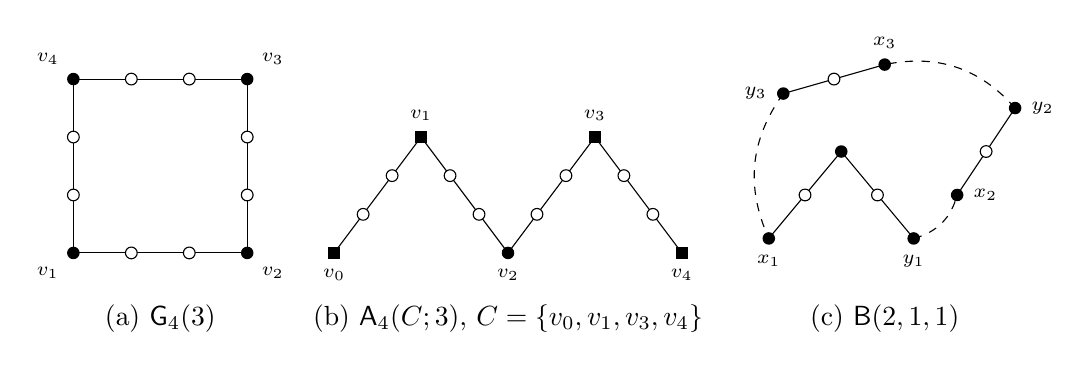
\begin{tikzpicture}[scale=0.92,
  junc/.style={circle,fill=black,inner sep=1.6pt},
  cjunc/.style={rectangle,fill=black,inner sep=2.1pt},
  free/.style={circle,draw=black,fill=white,inner sep=1.5pt},
  lab/.style={font=\scriptsize}]
\begin{scope}
  \draw (0,0)--(2.4,0)--(2.4,2.4)--(0,2.4)--cycle;
  \foreach \p in {(0.8,0),(1.6,0),(2.4,0.8),(2.4,1.6),(1.6,2.4),(0.8,2.4),(0,1.6),(0,0.8)} \node[free] at \p {};
  \node[junc,label={[lab]below left:$v_1$}] at (0,0) {};
  \node[junc,label={[lab]below right:$v_2$}] at (2.4,0) {};
  \node[junc,label={[lab]above right:$v_3$}] at (2.4,2.4) {};
  \node[junc,label={[lab]above left:$v_4$}] at (0,2.4) {};
  \node at (1.2,-0.9) {(a) $\GW_4(3)$};
\end{scope}
\begin{scope}[xshift=3.6cm]
  \draw (0,0)--(1.2,1.6)--(2.4,0)--(3.6,1.6)--(4.8,0);
  \foreach \p in {(0.4,0.533),(0.8,1.067),(1.6,1.067),(2.0,0.533),(2.8,0.533),(3.2,1.067),(4.0,1.067),(4.4,0.533)} \node[free] at \p {};
  \node[cjunc,label={[lab]below:$v_0$}] at (0,0) {};
  \node[cjunc,label={[lab]above:$v_1$}] at (1.2,1.6) {};
  \node[junc,label={[lab]below:$v_2$}] at (2.4,0) {};
  \node[cjunc,label={[lab]above:$v_3$}] at (3.6,1.6) {};
  \node[cjunc,label={[lab]below:$v_4$}] at (4.8,0) {};
  \node at (2.4,-0.9) {(b) $\FA_4(C;3)$, $C=\{v_0,v_1,v_3,v_4\}$};
\end{scope}
\begin{scope}[xshift=9.6cm,yshift=0.2cm]
  \draw (0,0)--(1.0,1.2)--(2.0,0);
  \node[free] at (0.5,0.6) {}; \node[free] at (1.5,0.6) {};
  \node[junc,label={[lab]below:$x_1$}] at (0,0) {};
  \node[junc] at (1.0,1.2) {};
  \node[junc,label={[lab]below:$y_1$}] at (2.0,0) {};
  \draw (2.6,0.6)--(3.4,1.8); \node[free] at (3.0,1.2) {};
  \node[junc,label={[lab]right:$x_2$}] at (2.6,0.6) {};
  \node[junc,label={[lab]right:$y_2$}] at (3.4,1.8) {};
  \draw (1.6,2.4)--(0.2,2.0); \node[free] at (0.9,2.2) {};
  \node[junc,label={[lab]above:$x_3$}] at (1.6,2.4) {};
  \node[junc,label={[lab]left:$y_3$}] at (0.2,2.0) {};
  \draw[dashed] (2.0,0) to[bend right=30] (2.6,0.6);
  \draw[dashed] (3.4,1.8) to[bend right=30] (1.6,2.4);
  \draw[dashed] (0.2,2.0) to[bend right=30] (0,0);
  \node at (1.6,-1.1) {(c) $\FB(2,1,1)$};
\end{scope}
\end{tikzpicture}
\caption{Schematic pictures of $\GW_4(3)$, of $\FA_4(C;3)$ with $C=\{v_0,v_1,v_3,v_4\}$, and of $\FB(2,1,1)$. Filled marks are junctions and open circles are freely added points; segments indicate the edge lines. In (b) the junctions in $C$ are drawn as squares. In (c) the dashed arcs join the three gap pairs $\{y_1,x_2\},\{y_2,x_3\},\{y_3,x_1\}$, which are the parallel pairs of the dual $\Gamma$ of the junction matroid. Ranks and dependencies are those of Definition~\ref{def:families}; the drawings are not geometric realizations.}
\label{fig:models}
\end{figure}


Thus $|\GW_r(t)|=rt$, $|\FA_r(C;t)|=(r+1)+r(t-1)=rt+1$, and $\FB(a,b,c)$ has rank $r=k+1\ge4$ and $(k+3)+k=2r+1$ elements. By Lemma~\ref{lem:unique}(b) these matroids do not depend on the order in which the interior points are added. The circuits of $J$ in (c) are the complements in the set of terminals of the three hyperplanes of $\Gamma$, namely
\begin{equation}\label{eq:Bcircuits}
D_1=\{x_1,y_2,x_3,y_3\},\quad D_2=\{x_1,y_1,x_2,y_3\},\quad D_3=\{y_1,x_2,y_2,x_3\},
\end{equation}
and the nonterminal junctions are coloops of $J$. In particular $J$ is simple and has no triangle. The matroid $J_C$ in (b) is simple, since $|C|\ge3$, and it has a triangle only when $|C|=3$.

\begin{lemma}[Lines of the models]\label{lem:modellines}
Let $r\ge3$.
\begin{enumerate}[label=\textup{(\alph*)}]
\item The long lines of $\GW_r(t)$ are the $r$ \emph{edge lines} $E_i=\{v_i,v_{i+1}\}\cup F_i$, where $F_i$ is the set of interior points on the edge $\{v_i,v_{i+1}\}$; each has $t+1$ points.
\item The long lines of $\FA_r(C;t)$ are the $r$ edge lines $E_i=\cl(\{v_i,v_{i+1}\})$, $0\le i\le r-1$, together with the set $C$ when $|C|=3$ and $C$ contains no edge. The edge line $E_i$ equals $\{v_i,v_{i+1}\}\cup F_i$ and has $t+1$ points, except when $|C|=3$ and $\{v_i,v_{i+1}\}\subseteq C$, in which case $E_i=C\cup F_i$ has $t+2$ points and is called \emph{heavy}. There is at most one heavy edge line.
\item The long lines of $\FB(a,b,c)$ are its $k=r-1$ edge triangles.
\end{enumerate}
\end{lemma}

\begin{proof}
This follows from Lemma~\ref{lem:triangles}, once we note that the models are simple (their cores are simple, and a free point is not parallel to anything since it is not spanned by a single element). The free matroid has no long lines and $\cl(\{v_i,v_{i+1}\})=\{v_i,v_{i+1}\}$ in it. In $J_C$ the only possible long line is $C$ when $|C|=3$, and $\cl_{J_C}(\{v_i,v_{i+1}\})$ equals $C$ if $|C|=3$ and $v_i,v_{i+1}\in C$, and $\{v_i,v_{i+1}\}$ otherwise. If $|C|=3$, then $C=\{v_0,v_j,v_r\}$ contains an edge only if $j\in\{1,r-1\}$, and since $r\ge3$ at most one of the edges $\{v_0,v_1\}$ and $\{v_{r-1},v_r\}$ lies in $C$. The core $J$ of (c) has no long lines.
\end{proof}

We call an edge line of $\FA_r(C;t)$ \emph{light} if it is not heavy. When $|C|=3$ and $C$ contains an edge, we say that $\FA_r(C;t)$ is \emph{heavy}. Since $v_0$ is then freely placed in $J_C$ on the pair formed by the other two elements of $C$, Lemma~\ref{lem:unique}(b) shows the following.

\begin{lemma}\label{lem:heavywhirl}
Let $r\ge3$. A heavy matroid $\FA_r(C;t)$ is the free extension of a basis $w_1,\dots,w_r$ in which $t-1$ interior points are added on each of the edges $\{w_i,w_{i+1}\}$, $1\le i\le r-1$, and $t$ interior points are added on the edge $\{w_r,w_1\}$. Conversely, every such free extension is a heavy member of Family~$\FA$. It is isomorphic to $W(r,2t)^+$.
\end{lemma}

\begin{proof}
By symmetry let $C=\{v_0,v_1,v_r\}$. In $J_C$ the junctions $v_1,\dots,v_r$ form a basis and $v_0\in\cl(X)$ holds exactly when $\{v_1,v_r\}\subseteq\cl(X)$, so $J_C$ is the principal extension of this basis on $\{v_r,v_1\}$. The interior points on $\{v_0,v_1\}$ are freely placed on the same line, which is also spanned by $\{v_r,v_1\}$. Put $w_i=v_i$ for $1\le i\le r$ and regard $v_0$ as an interior point of $\{w_r,w_1\}$; Lemma~\ref{lem:unique}(b) gives the first statement. The converse follows by reading the same argument backwards, choosing one of the $t$ interior points of $\{w_r,w_1\}$ as $v_0$, and the last statement follows from the definition of $W(r,2t)^+$.
\end{proof}

For $s\ge3$ we call a member of Family~$\FA$ of rank $s$ a \emph{heavy cycle} if it is heavy, and a \emph{light path} otherwise. By Lemmas~\ref{lem:modellines} and~\ref{lem:heavywhirl}, the edge lines of a light path form a path of $s$ lines with $t+1$ elements each, and those of a heavy cycle form a cycle of $s$ lines, one of which has $t+2$ elements.

We use the word \emph{interior point} for the freely added elements of a model, and also, in Section~\ref{sec:positroids}, for the elements of a cyclic interval other than its endpoints. In the natural order defined below, every freely added element is an interior point of its edge line, but the converse can fail: in a heavy member of Family~$\FA$, the junction $v_0$ lies between $v_r$ and the points freely added on $\{v_0,v_1\}$, so it is an interior point of the heavy line. Lemma~\ref{lem:adapted} below provides presentations in which the two notions agree.

\subsection{Positroid orders of the models}

\begin{lemma}[Free insertion]\label{lem:insert}
Let $M$ be a positroid with a positroid order in which the independent elements $a,b$ are cyclically consecutive. Then $M+_{ab}f$ is a positroid, and inserting $f$ between $a$ and $b$ gives a positroid order of it.
\end{lemma}

\begin{proof}
After a cyclic shift we may assume that $b$ immediately follows $a$ in the linear order. Let $A$ be a matrix representing $M$ whose maximal minors are nonnegative, with columns $a,b$ in particular. For every flat $F$ of $M$ with $\{a,b\}\not\subseteq F$, the subspace $\operatorname{span}(F)\cap\operatorname{span}(a,b)$ has dimension at most one. Choose $\alpha,\beta>0$ such that $x=\alpha a+\beta b$ avoids these finitely many subspaces, and insert the column $x$ between $a$ and $b$. A maximal minor containing $x$ equals $\alpha$ times the minor with $a$ in the position of $x$ plus $\beta$ times the minor with $b$ in that position. Each of these is zero if the column is repeated, and otherwise it is a maximal minor of $A$ with its columns in the original order, because no column lies between $a$ and the position of $x$, or between that position and $b$. Hence all maximal minors are nonnegative. For $X\subseteq E(M)$ with $F=\cl_M(X)$, we have $x\in\operatorname{span}(X)$ if and only if $\{a,b\}\subseteq F$, so the new matrix represents $M+_{ab}f$.
\end{proof}

\begin{corollary}\label{cor:positroidmodels}
Each matroid of Definition~\ref{def:families} is a positroid. A positroid order is obtained by listing the junctions in the order $v_1,\dots,v_r$ for $\GW_r(t)$, $v_0,\dots,v_r$ for $\FA_r(C;t)$, and $P_1,P_2,P_3$ (each path in order from $x_i$ to $y_i$) for $\FB(a,b,c)$, and inserting the interior points of each edge between its two junctions. We call this the \emph{natural order}.
\end{corollary}

\begin{proof}
The cores are positroids in the stated junction orders. This is clear for a free matroid. For $J_C$ it follows from Proposition~\ref{prop:positroid}(P2), as $C$ together with the singletons outside $C$ is a noncrossing partition and uniform matroids are positroids. For $\FB$, by (P1) it suffices to treat $\Gamma$. Shift the order cyclically so that it starts at $y_1$; the terminals then occur as $y_1,x_2,y_2,x_3,y_3,x_1$, with loops between them. Represent the loops by zero columns and the gap pairs $\{y_1,x_2\},\{y_2,x_3\},\{y_3,x_1\}$ by the vectors $(\cos\theta_j,\sin\theta_j)$, $j=1,2,3$, with $0<\theta_1<\theta_2<\theta_3<\pi$. Every $2\times2$ minor is $0$ or $\sin(\theta_j-\theta_i)$ with $i\le j$, hence nonnegative. Each edge is a pair of consecutive junctions, also for the edge $\{v_r,v_1\}$ of $\GW_r(t)$ in the cyclic sense. Insert the interior points of an edge $\{u,w\}$ one after another, each between the previously inserted point (or $u$) and $w$; since all of them lie on the line spanned by $u,w$, each step is the principal extension on $\{u,w\}$. Lemma~\ref{lem:insert} applies at every step.
\end{proof}

\subsection{Contracting interior points}

\begin{lemma}\label{lem:modelcontract}
Let $M$ be a simple free extension of a core $K$ by pairs $(f_j,P_j)_{j\le m}$, and let $f=f_1$ with $P_1=\{a,b\}$. Let $K^f=(K+_{ab}f)/f$, so that
\[
r_{K^f}(X)=r_K(X)-\big[\{a,b\}\subseteq\cl_K(X)\big]\qquad(X\subseteq E(K)),
\]
where $[\cdot]$ is $1$ if the condition holds and $0$ otherwise. Let $Z=E(K)-(\cl_K(\{a,b\})-a)$, and assume that $K^f|Z$ is simple. Then $M/f$ has exactly one nontrivial parallel class, namely $\cl_M(\{a,b\})-f$, and $\si(M/f)$, retaining $a$, is the free extension of $K^f|Z$ by the pairs $(f_j,P_j')$ for those $j\ge2$ with $P_j\not\subseteq\cl_K(\{a,b\})$, where $P_j'$ is obtained from $P_j$ by replacing an element of $\cl_K(\{a,b\})$, if there is one, by $a$.
\end{lemma}

\begin{proof}
By Lemma~\ref{lem:free}(d) the only nontrivial parallel class of $M/f$ is $\cl_M(\{a,b\})-f$, which by Lemma~\ref{lem:triangles} consists of the elements of $\cl_K(\{a,b\})$ and the $f_j$ with $P_j\subseteq\cl_K(\{a,b\})$. By Lemmas~\ref{lem:free}(a) and~\ref{lem:unique}(b), the restriction of $M$ to $E(K)\cup f$ is $K+_{ab}f$, so $(M/f)|E(K)=K^f$; the rank formula holds because $f\in\cl(X)$ exactly when $\{a,b\}\subseteq\cl_K(X)$. By Lemma~\ref{lem:free}(b), each remaining $f_j$ is freely placed on $P_j$ in $M/f$. If $P_j=\{u,w\}$ with $w\in\cl_K(\{a,b\})$, $w\ne a$, then $w$ is parallel to $a$ in $M/f$, so $\cl_{M/f}(\{u,w\})=\cl_{M/f}(\{u,a\})$ and, for $X$ not containing $w$, $w\in\cl_{M/f}(X)$ if and only if $a\in\cl_{M/f}(X)$; hence $f_j$ is freely placed on $P_j'$ in $(M/f)\backslash w$. Each $P_j'$ is independent in $K^f|Z$ because this matroid is simple, and Lemmas~\ref{lem:free}(a) and~\ref{lem:unique}(b) give the conclusion.
\end{proof}

\begin{lemma}[The cores after contraction]\label{lem:cores}
In the notation of Lemma~\ref{lem:modelcontract}:
\begin{enumerate}[label=\textup{(\alph*)}]
\item If $K$ is free on $\{v_1,\dots,v_r\}$ and $\{a,b\}=\{v_i,v_{i+1}\}$ with $a=v_i$, then $K^f|Z$ is free on $Z=\{v_1,\dots,v_r\}-v_{i+1}$.
\item Let $K=J_C$, $\{a,b\}=\{v_i,v_{i+1}\}$ with $a=v_i$, and suppose that $|C|\ge4$ or $\{v_i,v_{i+1}\}\not\subseteq C$. Then $Z=\{v_0,\dots,v_r\}-v_{i+1}$ and $K^f|Z=J_{C'}$, where $C'=C$ if $v_{i+1}\notin C$, $C'=(C-v_{i+1})\cup v_i$ if $v_{i+1}\in C$ and $v_i\notin C$, and $C'=C-v_{i+1}$ if $v_i,v_{i+1}\in C$. In each case $|C'|\ge3$, and $C'$ contains the first and last junction of the path $v_0,\dots,v_i,v_{i+2},\dots,v_r$.
\item Let $K=J_C$ with $C=\{v_0,v_1,v_r\}$, $r\ge3$, and $\{a,b\}=\{v_1,v_0\}$ with $a=v_1$. Then $Z=\{v_1,\dots,v_{r-1}\}$ and $K^f|Z$ is free.
\item Let $K=J$ be the core of $\FB(a,b,c)$ and let $\{u,w\}$ be an edge with $w$ nonterminal, $u$ retained. Then $K^f|Z=J\backslash w$, and $(J\backslash w)^*=\Gamma\backslash w$.
\item Let $K=J$ be the core of $\FB(a,b,c)$, let $P_1$ have a single edge $\{x_1,y_1\}$, and retain $x_1$. Put $T=\{x_2,y_2,x_3,y_3\}$. Then $K^f|(Z-x_1)=J_{T}$ on the junctions of $P_2$ and $P_3$ \textup{(}that is, $T$ is a circuit and all other junctions are coloops\textup{)}, and $x_1$ is freely placed on $\{x_2,y_3\}$ in $K^f|Z$.
\end{enumerate}
\end{lemma}

\begin{proof}
In each case $\cl_K(\{a,b\})=\{a,b\}$ except in (c), where it is $C$; this gives $Z$. For $X\subseteq Z$ we compute $\delta(X)=[\{a,b\}\subseteq\cl_K(X)]$.

(a) Since $v_{i+1}\notin X$ and $K$ is free, $\delta(X)=0$.

(b) If $v_{i+1}\notin C$, it is a coloop of $J_C$, so $\delta(X)=0$ and $K^f|Z=J_C\backslash v_{i+1}=J_C|Z$, which is $J_{C}$ on $Z$. If $v_{i+1}\in C$, then $v_{i+1}\in\cl(X)$ if and only if $C-v_{i+1}\subseteq X$, while $v_i\in\cl(X)$ if and only if $v_i\in X$, because the alternative $C-v_i\subseteq X$ would require $v_{i+1}\in X$. Hence $\delta(X)=1$ exactly when $C'\subseteq X$, where $C'=(C-v_{i+1})\cup v_i$. Since $Z$ spans $J_C$, the matroid $K^f|Z$ has $r$ elements and rank $r-1$, so it has exactly one circuit, every element outside it being a coloop; the formula shows that $C'$ is dependent while its proper subsets are independent. The size and end conditions follow from the hypotheses, from $v_0,v_r\in C$, and from $v_i\in C'$ whenever $v_{i+1}=v_r$.

(c) For $X\subseteq Z$, $v_0\in\cl_{J_C}(X)$ would require $v_r\in X$. Hence $\delta(X)=0$, and $J_C|Z$ is free.

(d) As $w$ is a coloop of $J$, $\delta(X)=0$ for $X\subseteq Z$. A coloop of $J$ is a loop of $\Gamma$, and $(J\backslash w)^*=\Gamma/w=\Gamma\backslash w$.

(e) By~\eqref{eq:Bcircuits}, every circuit of $J$ contains $x_1$ or $y_1$. Let $X\subseteq Z-x_1$. Then $X$ is independent in $J$; moreover $x_1\in\cl_J(X)$ if and only if $\{y_2,x_3,y_3\}\subseteq X$, and $y_1\in\cl_J(X)$ if and only if $\{x_2,y_2,x_3\}\subseteq X$. Hence $\delta(X)=[T\subseteq X]$ and $r_{K^f}(X)=|X|-[T\subseteq X]$, which proves the first claim. For the second, $X\cup x_1$ contains no circuit other than possibly $D_1$, so
\[
r_{K^f}(X\cup x_1)=|X|+1-\big[\{y_2,x_3,y_3\}\subseteq X\big]-\big[\{x_2,y_3\}\subseteq X\ \text{or}\ \{x_2,y_2,x_3\}\subseteq X\big].
\]
Comparing with $r_{K^f}(X)$, we find that $x_1\in\cl_{K^f}(X)$ holds exactly in the following cases: $T\subseteq X$; $\{y_2,x_3,y_3\}\subseteq X$ and $x_2\notin X$; or $\{y_2,x_3,y_3\}\not\subseteq X$ and ($\{x_2,y_3\}\subseteq X$ or $\{x_2,y_2,x_3\}\subseteq X$). In the second case $r_{K^f}(X\cup x_2)=|X|=r_{K^f}(X)$, so $x_2\in\cl_{K^f}(X)$ and $y_3\in X$. In the third case, if $y_3\notin X$, then $\{x_2,y_2,x_3\}\subseteq X$ and $r_{K^f}(X\cup y_3)=|X|$, so $y_3\in\cl_{K^f}(X)$. Thus $x_1\in\cl_{K^f}(X)$ implies $\{x_2,y_3\}\subseteq\cl_{K^f}(X)$, and taking $X=\{x_2,y_3\}$ shows $x_1\in\cl_{K^f}(\{x_2,y_3\})$.
\end{proof}

\begin{proposition}[The models]\label{prop:sufficiency}
Let $t\ge2$.
\begin{enumerate}[label=\textup{(\alph*)}]
\item For $r\ge2$, $\GW_r(t)$ is a $3$-connected positroid of rank $r$ with $rt$ elements and $q(\GW_r(t))=2t$. For $r\ge3$, contracting an interior point and simplifying gives $\GW_{r-1}(t)$, with loss $t$.
\item For $r\ge2$, every $\FA_r(C;t)$ is a $3$-connected positroid of rank $r$ with $rt+1$ elements and $q=2t+1$. For $r\ge3$, contracting an interior point of a light edge line and simplifying gives a member of Family~$\FA$ of rank $r-1$, with loss $t$; contracting an interior point of the heavy edge line gives $\GW_{r-1}(t)$, with loss $t+1$.
\item Every $\FB(a,b,c)$ is a $3$-connected positroid of rank $r=a+b+c+1$ with $2r+1$ elements and $q=5$. Contracting an interior point on a path with at least two edges and simplifying gives the matroid $\FB$ in which that path is shortened by one edge; contracting the interior point of a path with one edge, say $P_1$, gives $\FA_{r-1}(T;2)$ on the path that runs from $y_2$ backwards along $P_2$ to $x_2$, then along a new edge $\{x_2,y_3\}$ whose interior point is $x_1$, then backwards along $P_3$ from $y_3$ to $x_3$, with $T=\{x_2,y_2,x_3,y_3\}$. The loss is $2$.
\item In each of these matroids of rank at least three, every edge line is a nonseparating long line. If $C$ is the additional line of Lemma~\textup{\ref{lem:modellines}(b)}, then $M/C$ is disconnected.
\end{enumerate}
Consequently, all these matroids are $3$-connected positroids without a $U_{2,\ell+2}$-minor and with $tr+\varepsilon$ elements, where $\ell=2t-1$ in \textup{(a)}, $\ell=2t$ in \textup{(b)}, and $\ell=4$ in \textup{(c)}.
\end{proposition}

\begin{proof}
Positroid membership is Corollary~\ref{cor:positroidmodels} for rank at least three; the members of rank two are uniform matroids, which are positroids (Section~\ref{sec:positroids}). The cardinalities were noted after Definition~\ref{def:families}. By Lemma~\ref{lem:modellines} and Lemma~\ref{lem:free}(d), every interior point lies on exactly one long line, namely its edge line, so by~\eqref{eq:loss} its loss is the size of that line minus one.

\emph{Contractions.} The descriptions of the contractions follow from Lemmas~\ref{lem:modelcontract} and~\ref{lem:cores}; in each case below, the matroid $K^f|Z$ of Lemma~\ref{lem:modelcontract} is simple, being a free matroid, a matroid $J_{C'}$ with $|C'|\ge3$, the simple matroid $J\backslash w$, or $J_T$ with one further freely placed element: for (a) use Lemma~\ref{lem:cores}(a), which yields a free core on $r-1$ junctions whose edges again form a cycle (for $r=3$ the two remaining edges span the same line, which then carries $2+2(t-1)=2t$ points, giving $U_{2,2t}$); for a light edge line in (b) use Lemma~\ref{lem:cores}(b); for the heavy line in (b) use Lemma~\ref{lem:cores}(c), noting that after replacing $v_r$ by $v_1$ the edges form the cycle $v_1,\dots,v_{r-1}$; for (c) use Lemma~\ref{lem:cores}(d) and (e).

\emph{Three-connectivity.} We induct on the rank. The rank-two members $\GW_2(t)=U_{2,2t}$ and $\FA_2(C;t)=U_{2,2t+1}$ (all three junctions form the circuit $C$, and both edges span the whole line) are $3$-connected because $2t\ge4$. Let $M$ be a model of rank $r\ge3$; in Family~$\FB$ we induct on $a+b+c$, the base case being covered because every contraction of $\FB(1,1,1)$ lies in Family~$\FA$. Choose an interior point $f$ on an edge line $E$ that is light if $M$ is in Family~$\FA$. By the contraction statements and induction, $\si(M/f)$ is $3$-connected. By Lemma~\ref{lem:reconstruct} it suffices to check that $E(M)-E$ spans $M$; since every interior point lies in the closure of its two junctions, it suffices that $E(M)-E$ spans the two junctions $u,w$ of $E$. If $u$ lies on a second edge $\{u,u'\}$ with $u'\notin E$, then $u\in\cl(\{u',g\})$ for an interior point $g$ of that edge. In $\GW_r(t)$ every junction is of this kind. In $\FA_r(C;t)$ this handles every junction of $E$ except $v_0$ or $v_r$ when $E$ is the first or last edge line; such an end junction lies in $C$, and is spanned by the other elements of $C$, all of which are spanned by $E(M)-E$. In $\FB$, a nonterminal junction is handled as above, and a terminal junction $u$ is spanned by $D-u$ for a circuit $D$ of $J$ from~\eqref{eq:Bcircuits} that contains $u$ but not the other junction of $E$ when that junction is also terminal; such a $D$ exists, and when the other junction is nonterminal it lies in no circuit of $J$ at all. In every case the other junctions used are already spanned by $E(M)-E$.

\emph{The parameter $q$.} Every junction lies on an edge line with an interior point, so by Lemmas~\ref{lem:qrec}(b) and~\ref{lem:weakmap}, for a model $M$ of rank at least three $q(M)$ is the maximum of $q(\si(M/f))$ over the interior points $f$. By induction on the rank, using the contraction statements, we obtain $q(\GW_r(t))=q(U_{2,2t})=2t$, $q(\FA_r(C;t))=\max\{2t+1,2t\}=2t+1$ (the second value arising only from the heavy line), and $q(\FB)=5$, since all contractions of $\FB$ lie in Family~$\FB$ or in Family~$\FA$ with $t=2$.

\emph{Nonseparating lines.} In rank three every proper long line is nonseparating. In rank at least four, every edge line contains an interior point whose simplified contraction is $3$-connected, so it is nonseparating by Lemma~\ref{lem:contractornonsep}. If $|C|=3$ and $C$ contains no edge, then $C=\{v_0,v_j,v_r\}$ with $2\le j\le r-2$ is a connected flat that is not a cyclic interval of the natural order, because interior points lie between $v_0$ and $v_j$ and between $v_j$ and $v_r$; by Proposition~\ref{prop:positroid}(P4), $M/C$ is disconnected.

The final assertion follows since $q=2t=\ell+1$ in (a), $q=2t+1=\ell+1$ in (b) and $q=5=\ell+1$ in (c).
\end{proof}

\subsection{Recognizing the models}

\begin{lemma}[Recognition]\label{lem:recognition}
Let $M$ be a simple positroid of rank $r\ge3$ with a positroid order, and let $L_1,\dots,L_r$ be long lines of $M$ that are cyclic intervals, cover $E(M)$, pairwise meet in at most one point, and whose intersection graph is a cycle or a path, with $L_i,L_{i+1}$ adjacent.
\begin{enumerate}[label=\textup{(\alph*)}]
\item If the graph is a cycle, its $r$ intersection points form a basis, and $M$ is the free extension of this basis with $|L_i|-2$ interior points on the edge formed by the two intersection points on $L_i$. If all $L_i$ have $t+1$ points, then $M=\GW_r(t)$ with these junctions; if one has $t+2$ points and the others $t+1$, then $M$ is a heavy member of Family~$\FA$.
\item If the graph is a path, let $v_i$ be the intersection point of $L_i$ and $L_{i+1}$ for $1\le i\le r-1$, and let $v_0$ and $v_r$ be the endpoints of $L_1$ and $L_r$ that are not intersection points. If $M$ is $3$-connected and every $L_i$ has $t+1$ points, then the restriction of $M$ to $V=\{v_0,\dots,v_r\}$ is $J_C$ for a set $C$ with $|C|\ge3$ and $v_0,v_r\in C$, and $M=\FA_r(C;t)$ with these junctions.
\end{enumerate}
In both cases the junctions are exactly the endpoints of the intervals $L_i$, and the interior points are exactly the interior points of these intervals.
\end{lemma}

\begin{proof}
By Lemma~\ref{lem:intervals}, every intersection point is an endpoint of both lines, no point lies on three lines, and an interior point of some $L_i$ lies on no other $L_k$. In (a), the two intersection points on $L_i$ are distinct, so they are the two endpoints of $L_i$; in (b), the points $v_{i-1},v_i$ are the two endpoints of $L_i$, also for $i=1$ and $i=r$. Thus each $L_i$ is spanned by its two endpoints, the junctions span $E(M)$, and by Lemma~\ref{lem:interiorfree} every other point of $L_i$ is freely placed on the pair of endpoints of $L_i$. A junction lying on $L_i$ is an intersection point of $L_i$ with another line, or one of $v_0,v_r$, and hence is an endpoint of $L_i$; so $L_i$ contains exactly two junctions and $|L_i|-2$ interior points. In (a) the $r$ junctions span the rank-$r$ matroid and so form a basis; Lemma~\ref{lem:unique}(b) and Lemma~\ref{lem:heavywhirl} give the assertions. In (b) the $r+1$ junctions span, so $M|V$ has exactly one circuit $C$, the other junctions being coloops of $M|V$, and $|C|\ge3$ as $M$ is simple. If $v_0\notin C$, put $X=L_1-v_1$. Then $r(X)=2$, and $E(M)-X$ is spanned by $V-v_0$, which has rank $r-1$ because $v_0$ is a coloop of $M|V$; thus $\lam_M(X)\le1$ with $|X|\ge2$ and $|E(M)-X|\ge2$, contradicting $3$-connectivity. Similarly $v_r\in C$. Lemma~\ref{lem:unique}(b) gives $M=\FA_r(C;t)$.
\end{proof}

\begin{lemma}[Presentations adapted to a positroid order]\label{lem:adapted}
Let $N$ be a matroid isomorphic to a model of rank $s\ge3$, and fix any positroid order of $N$.
\begin{enumerate}[label=\textup{(\alph*)}]
\item If $N\cong\GW_s(t)$, its nonseparating long lines are $s$ lines of size $t+1$ that form a cycle and cover $E(N)$, and $N=\GW_s(t)$ with junctions the endpoints of these lines in the given order.
\item If $N$ is isomorphic to a member of Family~$\FA$, its nonseparating long lines are the images of the edge lines. If the member is heavy, they form a cycle with one line of size $t+2$; otherwise they form a path of $s$ lines of size $t+1$, and $N=\FA_s(C';t)$ for some $C'$, with junctions the endpoints of these lines in the given order. In the latter case, $N$ has at most one further long line; it has three points, and it is not a cyclic interval of the given order.
\item If $N$ is isomorphic to $\FB(a,b,c)$, its long lines are $s-1$ nonseparating triangles. In each triangle, the interior point in the given order is the constructed interior point, and $N=\FB(a',b',c')$ with paths $P_1,P_2,P_3$ that occur in this cyclic order and with $x_i,y_i$ the first and last junctions of $P_i$ in the given order.
\end{enumerate}
In every case, each point of $N$ is either a junction, which is an endpoint of every nonseparating long line containing it, or an interior point of exactly one nonseparating long line, and the nonseparating long lines are cyclic intervals of the given order.
\end{lemma}

\begin{proof}
By Proposition~\ref{prop:sufficiency}(d) and Lemma~\ref{lem:modellines}, the nonseparating long lines of $N$ are the images of the edge lines, and their incidence structure is as stated: in Family~$\FA$, consecutive edge lines meet in a junction, nonconsecutive ones are disjoint, and in the heavy case the heavy line $E_0=C\cup F_0$ also meets $E_{s-1}$ in $v_s$. They are cyclic intervals by Proposition~\ref{prop:positroid}(P4), and they cover $E(N)$. Lemma~\ref{lem:recognition} gives (a), and (b) except for the last sentence. If $N$ has a long line $X$ other than the edge lines, then by Lemma~\ref{lem:modellines} applied to the presentation just obtained, $X=C'$ consists of three junctions $v_0,v_j,v_s$ with $2\le j\le s-2$, and it is not a cyclic interval, because interior points lie between $v_0$ and $v_j$ and between $v_j$ and $v_s$.

For (c), let $T=\{u,f,w\}$ be an edge triangle with constructed interior point $f$, that is, $f$ is the element added on the edge $\{u,w\}$ in Definition~\ref{def:families}(c). By Lemma~\ref{lem:interiorfree}, the interior point of $T$ in the given order is freely placed on $T$. We show that $u$ is not freely placed on $T$ in $N$; the same holds for $w$. If $u$ is nonterminal, it lies on a second triangle $\{u,f',u'\}$, and $u\in\cl(\{f',u'\})$ while $T\not\subseteq\cl(\{f',u'\})$. If $u$ is terminal, note that $u$ lies in exactly the two circuits among $D_1,D_2,D_3$ whose omitted gap pair does not contain $u$; if $w$ is also terminal, then $u,w$ lie in different gap pairs, so in any case we can choose $D\in\{D_1,D_2,D_3\}$ with $u\in D$ and $w\notin D$. Then $u\in\cl(D-u)$, but $w\notin\cl_J(D-u)$: if $w$ is nonterminal it is a coloop of $J$, and if $w$ is terminal, a circuit of $J$ through $w$ inside $(D-u)\cup w$ would be the four-element set $(D-u)\cup w$, which is the set of terminals other than $u$ and the element of $G-w$, where $G$ is the gap pair omitted by $D$; as these two elements lie in different gap pairs, this set is none of $D_1,D_2,D_3$. Hence the interior point of $T$ in the given order is $f$, so the junctions, the edges and the paths (the components of the intersection graph of the triangles) are determined by $N$ and the order. Consecutive triangles of a path meet in a common endpoint and nonconsecutive ones are disjoint; inductively, the union of the first $k$ triangles of a path is a cyclic interval meeting the next triangle only in a common endpoint, and the union of two cyclic intervals meeting only in a common endpoint is a cyclic interval or the whole ground set. The latter is impossible because there are three paths, so the union of the triangles of each path is a cyclic interval. Let $P_1,P_2,P_3$ be the paths in their cyclic order, and let $x_i,y_i$ be the first and last junctions of $P_i$. The nonterminal junctions are loops of $\Gamma=(N|\{\text{junctions}\})^*$, and by Proposition~\ref{prop:positroid}(P1) the matroid $\Gamma$ deleted by its loops is a loopless positroid of rank two on $x_1,y_1,x_2,y_2,x_3,y_3$ in this cyclic order. Its three parallel classes have two elements each, lie in different paths, and are cyclic intervals; hence they are $\{y_1,x_2\},\{y_2,x_3\},\{y_3,x_1\}$. Lemma~\ref{lem:unique}(b) gives $N=\FB(a',b',c')$.

The final statement follows from the presentations and Lemma~\ref{lem:intervals}.
\end{proof}

From now on, whenever a matroid isomorphic to a model carries a positroid order, we use the presentation adapted to that order given by Lemma~\ref{lem:adapted}, and we speak of its junctions, interior points and edge lines accordingly.

\section{Equality constraints and the reconstruction setup}\label{sec:equality}

From now on $\ell\ge4$, and $t,\varepsilon$ are as in the introduction; thus $t\ge2$, and $t\ge3$ when $\ell$ is odd. We call a matroid \emph{extremal} (for $\ell$) if it is a $3$-connected positroid of some rank $r\ge2$ with no $U_{2,\ell+2}$-minor and with exactly $tr+\varepsilon$ elements. A nonseparating long line of size $t+1$ is \emph{light}, and one of size $t+2$ is \emph{heavy}; by Proposition~\ref{prop:sufficiency} and Lemma~\ref{lem:modellines} this agrees with the terminology for the models. By Proposition~\ref{prop:sufficiency}, every model of the appropriate parity is extremal.

\begin{lemma}[Equality constraints]\label{lem:equality}
Let $M$ be extremal of rank $r\ge3$.
\begin{enumerate}[label=\textup{(\alph*)}]
\item $q(M)=\ell+1=2t+\varepsilon$.
\item If $x\in E(M)$ and $\si(M/x)$ is $3$-connected, then $\delta_M(x)\ge t$, and $\si(M/x)$ is extremal if $\delta_M(x)=t$.
\item Every nonseparating long line of $M$ has at least $t+1$ elements.
\item $M$ has at least two nonseparating long lines.
\item Every nonseparating long line of $M$ has $t+1$ or $t+1+\varepsilon$ elements, and at most one of them has $t+2$ elements. In particular $M$ has a light nonseparating line.
\end{enumerate}
\end{lemma}

\begin{proof}
(a) Certainly $q(M)\le\ell+1$. If $q(M)\le\ell$, then $M$ has no $U_{2,\ell+1}$-minor, and Theorem~\ref{thm:bound} with $\ell-1\ge3$ in place of $\ell$ gives $|E(M)|\le(t-1)r+1<tr$ if $\ell=2t-1$, and $|E(M)|\le tr<tr+1$ if $\ell=2t$. Both contradict extremality.

(b) The matroid $\si(M/x)$ is a $3$-connected positroid of rank $r-1\ge2$ without a $U_{2,\ell+2}$-minor, so it has at most $t(r-1)+\varepsilon$ elements by Theorem~\ref{thm:bound}. Hence $\delta_M(x)\ge t$, with equality exactly when $\si(M/x)$ is extremal.

(c) A nonseparating long line $L$ is a cyclic interval by Proposition~\ref{prop:positroid}(P4); an interior point $e$ of $L$ is free by Lemma~\ref{lem:interiorfree}, and Lemma~\ref{lem:freecontract} and (b) give $|L|-1=\delta_M(e)\ge t$.

(d) Suppose that $r\ge4$. By Lemma~\ref{lem:wu}, applied to any line, there is $e_0$ with $\si(M/e_0)$ $3$-connected. As $\delta_M(e_0)\ge t\ge2$, the element $e_0$ lies on a long line $K_0$ by~\eqref{eq:loss}, and $K_0$ is nonseparating by Lemma~\ref{lem:contractornonsep}. Lemma~\ref{lem:wu} applied to $K_0$ gives $e\notin K_0$ with $\si(M/e)$ $3$-connected, and as before $e$ lies on a nonseparating long line $K\ne K_0$. Suppose that $r=3$. Then every proper long line is nonseparating, and $|E(M)|=3t+\varepsilon\ge6$. If an element $x$ lies on no long line, then $M/x$ is a simple matroid of rank two with at least five elements, hence $3$-connected, and $\delta_M(x)=1<t$, contrary to (b). Thus there is a long line $L$, and an element outside $L$ lies on a second long line.

(e) If $L\ne L'$ are nonseparating long lines, then Lemma~\ref{lem:twolines}, (a) and (c) give $|L|+|L'|\le 2t+2+\varepsilon$ and $|L|,|L'|\ge t+1$. By (d), every nonseparating long line $L$ has such a partner $L'$, so $|L|\le t+1+\varepsilon$; and two lines of size $t+2$ would violate the inequality.
\end{proof}

\begin{lemma}[Rank three]\label{lem:rank3}
Let $M$ be an extremal matroid of rank three. Then $M$ has exactly three long lines, they are nonseparating, they cover $E(M)$, and with respect to any positroid order one of the following holds.
\begin{enumerate}[label=\textup{(\roman*)}]
\item $\varepsilon=0$, the three lines have $t+1$ elements each and pairwise meet in three distinct points, and $M=\GW_3(t)$;
\item $\varepsilon=1$, the three lines have $t+1$ elements each and form a path, and $M=\FA_3(C;t)$ with $C$ the set of its four junctions \textup{(}the \emph{light path}\textup{)};
\item $\varepsilon=1$, the three lines have $t+2$, $t+1$, $t+1$ elements and pairwise meet in three distinct points, and $M$ is a heavy member of Family~$\FA$ \textup{(}the \emph{heavy cycle}\textup{)}.
\end{enumerate}
\end{lemma}

\begin{proof}
Fix a positroid order. All proper long lines are nonseparating, hence cyclic intervals of size at least $t+1\ge3$, and Lemma~\ref{lem:intervals} applies to them. Every element lies on a long line: otherwise contracting it would give a simple rank-two matroid with $3t+\varepsilon-1>2t+\varepsilon$ elements, contrary to Lemma~\ref{lem:equality}(a). Let $k$ be the number of long lines and $a$ the number of elements on two of them. No element lies on three long lines, and each line meets at most two others, at its endpoints, so $a\le k$. Hence $3t+\varepsilon=|E(M)|=\sum|L|-a\ge k(t+1)-k=kt$, and $k\le3$ because $t\ge2$. One line cannot cover a rank-three matroid. If two lines $L_1,L_2$ cover $E(M)$, then $|E(M)-L_1|\ge 3t+\varepsilon-(t+1+\varepsilon)\ge 2$ and $\lam_M(L_1)\le 2+2-3=1$, a $2$-separation. Thus $k=3$, and $\sum|L|=3t+\varepsilon+a$. By Lemma~\ref{lem:equality}(e), if $\varepsilon=0$ all three lines have $t+1$ elements and $a=3$; if $\varepsilon=1$, either all have $t+1$ elements and $a=2$, or the sizes are $t+2,t+1,t+1$ and $a=3$. When $a=3$ the intersection graph is a triangle, and the three intersection points are distinct because no point lies on three lines; when $a=2$ it is a path. Lemma~\ref{lem:recognition} identifies $M$; in (ii), the circuit $C$ has four elements because a three-element $C$ containing both ends of a path of three edges contains an edge, which would produce a heavy line.
\end{proof}

\begin{setup}\label{setup}
This setup is used to reconstruct an extremal matroid $M$ from a smaller extremal matroid $N$. Let $M$ be extremal of rank $r\ge3$ with a fixed positroid order. Let $L$ be a light nonseparating line of $M$, let $e$ be an interior point of $L$, and let $N=\si(M/e)$, where a point $p\in L-e$ is retained to represent the parallel class $L-e$; $N$ carries the induced order. By Lemmas~\ref{lem:interiorfree} and~\ref{lem:freecontract}, $e$ is freely placed on $L$, the class $L-e$ is the only nontrivial parallel class of $M/e$, and $N$ is $3$-connected; by Lemma~\ref{lem:equality}(b), $N$ is extremal of rank $r-1$. We identify $E(N)-p$ with $E(M)-L$. For $X\subseteq E(M)-L$,
\begin{equation}\label{eq:rankN}
r_N(X)=r_M(X\cup e)-1,\qquad r_N(X\cup p)=r_M(X\cup L)-1.
\end{equation}
In the induced order of $N$, the element $p$ occupies the position of the interval $L$: if $L$ is removed from the cyclic order of $M$ and $p$ is put in its place, the cyclic order of $N$ results.
\end{setup}

\begin{lemma}[Lifting a line that avoids $p$]\label{lem:liftB}
In Setup~\textup{\ref{setup}}, let $Q$ be a nonseparating long line of $N$ with $p\notin Q$. Then $Q$ is a nonseparating long line of $M$, it is a cyclic interval of $M$ with the same endpoints and interior points as in $N$, and $Q\cap L=\emptyset$.
\end{lemma}

\begin{proof}
By~\eqref{eq:rankN}, $r_M(Q\cup e)=3$. If $r_M(Q)=3$, then $e\in\cl_M(Q)$, freeness gives $L\subseteq\cl_M(Q)$, and~\eqref{eq:rankN} gives $p\in\cl_N(Q)=Q$, a contradiction. Hence $r_M(Q)=2$ and $e\notin\cl_M(Q)$. An element $x\in E(M)-L$ with $x\in\cl_M(Q)$ satisfies $x\in\cl_N(Q)=Q$. If $x\in(L-e)\cap\cl_M(Q)$, then $L=\cl_M(\{x,e\})\subseteq\cl_M(Q\cup e)$ and $p\in\cl_N(Q)$, again impossible. Thus $Q$ is a line of $M$.

The matroid $(M/e)/Q$ is obtained from $N/Q$ by adding the elements of $L-e$ other than $p$ as parallel copies of $p$, which is not a loop of $N/Q$ since $Q$ is a flat of $N$. Hence $(M/Q)/e$ is connected by Lemma~\ref{lem:basic}(a). Put $P=M/Q$. The element $e$ is a nonloop of $P$, and it is not a coloop of $P$ because $r_P(E(P)-e)=r_M(E(M)-e)-r_M(Q)=r(P)$. If $P=P_1\oplus P_2$ with nonempty $E(P_1),E(P_2)$ and $e\in E(P_1)$, then $E(P_1)\ne\{e\}$, since otherwise $e$ would be a coloop, and $P/e=(P_1/e)\oplus P_2$ would be disconnected. So $P$ is connected and $Q$ is nonseparating in $M$. Since $Q\cap L=\emptyset$ and $L$ is an interval, the cyclic order of $Q$ and of its complement is the same in $M$ and in $N$, so $Q$ has the same endpoints and interior points in both.
\end{proof}

\begin{lemma}[Commuting contractions]\label{lem:liftC}
In Setup~\textup{\ref{setup}}, let $Q$ be a nonseparating long line of $N$ with $p\notin Q$, and let $f$ be an interior point of $Q$. Then:
\begin{enumerate}[label=\textup{(\arabic*)}]
\item $f$ is freely placed on $Q$ in both $M$ and $N$, and in both $M/f$ and $N/f$ the only nontrivial parallel class is $Q-f$; neither has loops.
\item Let $M_1=\si(M/f)$ and $N_1=\si(N/f)$, formed with the same representative of $Q-f$. Then $M_1$ and $N_1$ are $3$-connected positroids with the induced orders, and $\delta_M(f)=\delta_N(f)=|Q|-1$.
\item $L$ is a line of $M_1$, the element $e$ is an interior point of $L$ in $M_1$ and is freely placed on $L$, $L$ is nonseparating in $M_1$, and $\si(M_1/e)=N_1$ with the same retained element $p$.
\end{enumerate}
If moreover $|Q|=t+1$, then $(M_1,L,e,N_1,p)$ is again an instance of Setup~\textup{\ref{setup}}, with $r(M_1)=r(M)-1$.
\end{lemma}

\begin{proof}
By Lemma~\ref{lem:liftB}, $Q$ is a nonseparating interval of $M$ with interior point $f$, and it is also one of $N$. Lemmas~\ref{lem:interiorfree} and~\ref{lem:freecontract} give (1) and (2); in $M$ the class $Q-f$ is disjoint from $L$, so $M_1$ can be formed retaining every element of $L$.

For (3), two elements $a,b\in L$ remain independent in $M/f$, since otherwise $\{a,b,f\}$ would be a triangle through $f$, which lies in $Q$ by Lemma~\ref{lem:free}(d). So $L$ has rank two in $M_1$. If $x\in E(M_1)-L$ lay in $\cl_{M_1}(L)$, then in $M/f/e=(M/e)/f$ the element $x$ would be parallel to $p$ or a loop; but in $N/f$ the class of $p$ is $\{p\}$ and there are no loops. Hence $L$ is a line of $M_1$. By Lemma~\ref{lem:free}(a),(b), $e$ is freely placed on $L$ in $M_1$. Both neighbours of $e$ in $M$ belong to $L$ and are retained, so $e$ is an interior point of $L$ in $M_1$. The matroid $M_1/e$ is a restriction of $(M/e)/f$, whose simplification is $\si(N/f)$; the classes $Q-f$ and $L-e$ do not merge because $p\notin Q$. With the same representatives, $\si(M_1/e)=N_1$. Since $N$ has the proper nonseparating line $Q$, we have $r(N)\ge3$, so $r(M_1)\ge3$. If $r(M_1)=3$, then $M_1/L$ is connected because it is loopless of rank one; if $r(M_1)\ge4$, Lemma~\ref{lem:contractornonsep} applies to $e$, since $\si(M_1/e)=N_1$ is $3$-connected. Finally, if $|Q|=t+1$ then $|E(M_1)|=tr+\varepsilon-t$, so $M_1$ is extremal of rank $r-1$, and $L$ is a light nonseparating line of it.
\end{proof}

Changing the representative within a parallel class changes a simplification only by relabelling one element, so all statements below about simplifications are independent of these choices; we always retain the whole of $L$ in contractions of $M$, and $p$ in contractions of $N$.

\begin{definition}\label{def:reduction}
Assume Setup~\ref{setup} and that $N$ is isomorphic to a model of rank at least three, equipped with the presentation adapted to its order (Lemma~\ref{lem:adapted}). A \emph{reduction sequence} is a sequence $f_1,\dots,f_m$ such that, writing $(M_0,N_0)=(M,N)$, the element $f_i$ is an interior point of a light nonseparating line $Q_i$ of $N_{i-1}$ with $p\notin Q_i$, and $M_i=\si(M_{i-1}/f_i)$, $N_i=\si(N_{i-1}/f_i)$; we require $r(N_{i-1})\ge3$ for $i\le m$. We write $Y=\{f_1,\dots,f_m\}$. For an element $x$ of $N$ that is not in $\{f_1,\dots,f_i\}$ and is not a loop of $N/\{f_1,\dots,f_i\}$, its \emph{image} in $N_i$ is the retained representative of the parallel class of $x$ in $N/\{f_1,\dots,f_i\}$; images in $M_i$ of elements of $M$ are defined in the same way.
\end{definition}

\begin{lemma}[Reduction]\label{lem:reduction}
Let $f_1,\dots,f_m$ be a reduction sequence. Then for each $i\le m$:
\begin{enumerate}[label=\textup{(\alph*)}]
\item $(M_i,L,e,N_i,p)$ is an instance of Setup~\textup{\ref{setup}}, $r(M_i)=r-i$, and $N_i$ is isomorphic to a model: to $\GW_{r-1-i}(t)$ if $N\cong\GW_{r-1}(t)$, to a member of Family~$\FA$ if $N$ is in Family~$\FA$, and to a member of Family~$\FA$ or $\FB$ if $N$ is in Family~$\FB$.
\item The set $Y$ is independent in $M$ and in $N$ and disjoint from $L$; $M_m$ is a simplification of $M/Y$, $N_m$ is a simplification of $N/Y$, and for $x,y\in E(M)-(L\cup Y)$ the elements $x,y$ are parallel in $M/Y$ if and only if they are parallel in $N/Y$. No element of $L$ is parallel in $M/Y$ to another element, and $p$ is parallel in $N/Y$ to no other element.
\item Let $E$ be a nonseparating long line of $N$ such that, for every $i$, $Q_i$ is not the closure in $N_{i-1}$ of the set of images of $E$. Then the elements of $E$ are pairwise nonparallel nonloops of $N/Y$, and if $r(N_i)\ge3$, the closure $E^{(i)}$ of the images of $E$ in $N_i$ is a nonseparating long line of $N_i$ with at most one element that is not an image of an element of $E$. If $E'$ is a second such line, then $E^{(i)}\ne E'^{(i)}$ whenever $r(N_i)\ge3$.
\item In \textup{(c)}, if all elements of $E$ are retained in each $N_i$ and $g$ is an interior point of $E$ whose two neighbours in $N$ belong to $E$, then for each $i$ with $r(N_i)\ge3$, $g$ is an interior point of $E^{(i)}$, it lies on no other nonseparating long line of $N_i$, $g\notin Y$, and the parallel class of $g$ in $N/Y$ is $\{g\}$.
\end{enumerate}
\end{lemma}

\begin{proof}
Part (a) follows by induction from Lemma~\ref{lem:liftC} and from the contraction descriptions in Proposition~\ref{prop:sufficiency}, applied to the adapted presentation of $N_{i-1}$, in which $f_i$, an interior point of $Q_i$ in the induced order, is a freely added point (Lemma~\ref{lem:adapted}). Part (b) follows by induction from Lemma~\ref{lem:liftC}(1): each $f_i$ is a nonloop of $M_{i-1}$ and of $N_{i-1}$, the class $Q_i-f_i$ is the only nontrivial class at step $i$ in both matroids, it is disjoint from $L$, and $p\notin Q_i$.

(c) We induct on $i$. The line $Q_i$ differs from the line $E^{(i-1)}$ (with $E^{(0)}=E$) and meets it in at most one element, so the images of $E$ remain pairwise nonparallel nonloops in $N_{i-1}/f_i$. By Lemma~\ref{lem:modelcontract} and Proposition~\ref{prop:sufficiency}, the edge lines of $N_i$ are the closures of the images of the edge lines of $N_{i-1}$ other than $Q_i$, together with one new edge line when $N_{i-1}$ is in Family~$\FB$ and $Q_i$ is a path of one edge. Hence $E^{(i)}$ is an edge line, and it is nonseparating by Proposition~\ref{prop:sufficiency}(d). An edge line of a model has at most $t+2$ elements, and $E$ has at least $t+1$ images, which gives the bound on extra elements. Suppose that $E^{(i)}=E'^{(i)}$ with $r(N_i)\ge3$. Passing from $N_{i-1}$ to $N_i$ identifies elements only within $Q_i-f_i$, and $Q_i$ meets each of $E^{(i-1)},E'^{(i-1)}$ in at most one element. If the two lines are disjoint, their union has at least $2t+2$ elements, of which at most one pair is identified; if they meet but not both meet $Q_i$, their union has at least $2t+1$ elements and none is identified. In both cases at least $2t+1>t+2$ distinct elements of $N_i$ lie on one line, which is impossible. Otherwise the three nonseparating lines $E^{(i-1)},E'^{(i-1)},Q_i$ pairwise meet. In the models the intersection graph of the nonseparating lines is a path, a disjoint union of paths, or a cycle of length equal to the rank (Lemma~\ref{lem:adapted}), so this happens only when $r(N_{i-1})=3$, that is, when $r(N_i)=2$.

(d) Since $g$ and its two neighbours are retained in $N_i$, they remain neighbours in the induced order, and they lie in $E\subseteq E^{(i)}$. Hence $g$ is an interior point of the cyclic interval $E^{(i)}$, and by Lemma~\ref{lem:intervals} it lies on no other nonseparating long line of $N_i$. In particular $g$ is never the element $f_{i+1}$, which is an interior point of a line $Q_{i+1}\ne E^{(i)}$, and $g$ never belongs to the nontrivial class $Q_{i+1}-f_{i+1}$; so its class in $N/Y$ is $\{g\}$.
\end{proof}

\begin{lemma}[Skewness]\label{lem:skew}
In Setup~\textup{\ref{setup}}, let $J$ be a long line of $N$ with $p\in J$, put $S=J-p$ and $F=L\cup S$. Then $F$ is a flat of rank three of $M$. If $Y\subseteq E(M)-(L\cup S)$ is independent in $N$ and $r_{N/Y}(S)=2$, then $Y$ is skew to $F$ in $M$, and $r_{M/Y}(X)=r_M(X)$ for every $X\subseteq F$.
\end{lemma}

\begin{proof}
By~\eqref{eq:rankN}, $r_M(S\cup e)=r_N(S)+1=3$. The flat $\cl_M(S\cup e)$ contains $L$ because $p\in\cl_N(S)$, and an element $x\in E(M)-L$ lies in it if and only if $x\in\cl_N(S)=J$. Thus $\cl_M(S\cup e)=F$. Next, $r_M(Y)\ge r_M(Y\cup e)-1=r_N(Y)=|Y|$, so $Y$ is independent in $M$, and $r_M(Y\cup F)=r_M(Y\cup S\cup e)=r_N(Y\cup S)+1=|Y|+3=r_M(Y)+r_M(F)$. For $X\subseteq F$, submodularity gives $r_M(X\cup Y)\ge r_M(X)+r_M(Y)$, whence $r_{M/Y}(X)=r_M(X)$.
\end{proof}

\begin{lemma}[An incident line]\label{lem:liftF}
In Setup~\textup{\ref{setup}}, let $J$ be a nonseparating long line of $N$ with $p\in J$, let $S=J-p$ and $F=L\cup S$. Then either $r_M(S)=3$ and $\cl_M(S)=F$, or $r_M(S)=2$ and $K=\cl_M(S)$ equals $S$ or $S\cup\{x\}$ for a single $x\in L$, and $M/K$ is connected.
\end{lemma}

\begin{proof}
By Lemma~\ref{lem:skew}, $F$ is a flat of rank three containing $S$. If $r_M(S)=3$ then $\cl_M(S)=F$. Let $r_M(S)=2$ and $K=\cl_M(S)\subseteq F$. If $K$ contained two elements of $L$, it would contain $L$ and then $F$, so $K\cap L$ has at most one element. Put $P=M/K$ and $T=L-K=F-K$. Then $r_P(T)=r_M(F)-r_M(K)=1$, the matroid $P$ is loopless since $K$ is a flat, and $\cl_P(T)=\cl_M(K\cup T)-K=F-K=T$. Thus $T$ is a full parallel class of the loopless matroid $P$. Moreover $P/T=M/F$, and for $X\subseteq E(M)-F$ we get from~\eqref{eq:rankN} that $r_{M/F}(X)=r_M(X\cup S\cup e)-3=r_N(X\cup J)-2=r_{N/J}(X)$, so $M/F=N/J$ is connected.

Suppose that $P=P_1\oplus P_2$ with both parts nonempty and $T\subseteq E(P_1)$. If $E(P_1)\ne T$, then $P_1/T$ has a nonloop element, and $P/T=(P_1/T)\oplus P_2$ is disconnected. Hence $E(P_1)=T$, and
\begin{align*}
\lam_M(T)&=r_M(T)+r_M(E(M)-T)-r(M)=2+\big(r_M(K)+r_P(E(P)-T)\big)-r(M)\\
&=2+(r(M)-1)-r(M)=1.
\end{align*}
Here $|T|\ge2$ and $|E(M)-T|\ge|S|\ge2$, contradicting $3$-connectivity. Thus $P$ is connected.
\end{proof}

\begin{lemma}[Heavy lines contain $p$]\label{lem:heavyprotect}
In Setup~\textup{\ref{setup}}, suppose that $\varepsilon=1$, that $N$ is isomorphic to a model of rank at least three, and that $p$ is an interior point of a nonseparating long line $J$ of $N$. Then every heavy line of $N$ contains $p$.
\end{lemma}

\begin{proof}
Suppose that $X$ is a heavy line of $N$ with $p\notin X$. Then $N$ is a heavy member of Family~$\FA$, and $X$ is its unique heavy line. We construct a reduction sequence in which $J$ and $X$ are never contracted, retaining all elements of $J$. Suppose $f_1,\dots,f_i$ have been chosen and $r(N_i)\ge3$. By Lemma~\ref{lem:reduction}(c),(d), the images of $X$ are $t+2$ pairwise distinct elements of the line $X^{(i)}$, which therefore equals this set of images and is the heavy line of $N_i$; $p\notin X^{(i)}$ because the class of $p$ is $\{p\}$; and $p$ is an interior point of $J^{(i)}$ and lies on no other nonseparating line. The model $N_i$ is heavy, so it has $r(N_i)-1\ge2$ light lines, at most one of which contains $p$. Choose a light line avoiding $p$ as $Q_{i+1}$. We stop when $r(N_m)=2$, so that $r(M_m)=3$. The images of $X$ in $M_m$ are $t+2$ distinct elements, by Lemma~\ref{lem:reduction}(b),(c); they are collinear, because $r_M(X)=2$ by Lemma~\ref{lem:liftB}; and they do not belong to $L$. By Lemma~\ref{lem:rank3}, a line of the extremal rank-three matroid $M_m$ with at least $t+2$ elements is the heavy line of the heavy cycle, so it equals the set of images of $X$ and is disjoint from $L$. But in the heavy cycle every two long lines meet. This contradiction proves the lemma.
\end{proof}

\begin{lemma}[Preserving an outer line]\label{lem:protected}
In Setup~\textup{\ref{setup}}, suppose that $N$ is isomorphic to a model of rank $s\ge3$, that $p$ is an interior point of a nonseparating long line $J$ of $N$, and that $Q\ne J$ is a light nonseparating line of $N$. Then there is a reduction sequence with contracted set $Y$ such that, with $M'=M_m$, $N'=N_m$ and $S=J-p$:
\begin{enumerate}[label=\textup{(\roman*)}]
\item $r(M')=3$, $r(N')=2$, and $M'$ contains every element of $L\cup S$; $L$ is a light line of $M'$;
\item $r_{N/Y}(S)=2$, so that $Y$ is skew to $F=L\cup S$ and $r_{M'}(X)=r_M(X)$ for all $X\subseteq F$;
\item the images in $M'$ of the elements of $Q$ form a set $Q_0$ of $t+1$ distinct collinear elements disjoint from $L$;
\item if $g\in S$ is an interior point of $J$, then $g\notin Q_0$.
\end{enumerate}
\end{lemma}

\begin{proof}
We choose $f_1,f_2,\dots$ so that neither $J$ nor $Q$ is contracted, retaining all elements of $J$; this is possible since the elements of $J$ remain pairwise nonparallel (Lemma~\ref{lem:reduction}(c)). Since $J$ is an interval and $p$ is an interior point of it, both neighbours of $p$ lie in $J$, so by Lemma~\ref{lem:reduction}(d) $p$ remains an interior point of $J^{(i)}$ and lies on no other nonseparating line of $N_i$. Suppose $f_1,\dots,f_i$ are chosen and $s_i=r(N_i)\ge3$. If $\varepsilon=1$, Lemma~\ref{lem:heavyprotect} applied to the instance $(M_i,L,e,N_i,p)$ shows that every heavy line of $N_i$ is $J^{(i)}$; in particular $Q^{(i)}$ is light, and $Q^{(i)}\ne J^{(i)}$ by Lemma~\ref{lem:reduction}(c). If $s_i\ge4$, the model $N_i$ has at least $s_i-1\ge3$ light lines, so there is a light line other than $J^{(i)}$ and $Q^{(i)}$; it avoids $p$. If $s_i=3$, then $N_i$ is $\GW_3(t)$, the light path or the heavy cycle; in the heavy cycle the heavy line is $J^{(i)}$. In all three cases there is a third light line, which avoids $p$. We contract an interior point of it, and stop when $r(N_m)=2$.

Part (i) follows from Lemma~\ref{lem:reduction}(a),(b) and the choice of representatives. The images of $J$ are $|J|\ge t+1$ pairwise nonparallel nonloops of $N/Y$, so $r_{N/Y}(S)=2$, and Lemma~\ref{lem:skew} gives (ii); $Y\cap S=\emptyset$ because the elements of $Y$ are interior points of lines other than $J^{(i)}$, and elements of $S$ lie on $J^{(i)}$. For (iii), the images of $Q$ are pairwise distinct by Lemma~\ref{lem:reduction}(b),(c), they lie outside $L$ by Lemma~\ref{lem:reduction}(b), and they are collinear in $M'$ because $r_M(Q)=2$ by Lemma~\ref{lem:liftB}. For (iv), the neighbours of an interior point $g\in S$ of $J$ lie in $J$, so by Lemma~\ref{lem:reduction}(d) and (b) the class of $g$ in $M/Y$ is $\{g\}$; since $g$ lies on no nonseparating line other than $J$, we have $g\notin Q$, and therefore $g$ is not the image of an element of $Q$.
\end{proof}

\section{Odd parameters}\label{sec:odd}

\begin{theorem}\label{thm:odd}
Let $\ell=2t-1$ with $t\ge3$, and let $r\ge2$. A matroid is extremal of rank $r$ if and only if it is isomorphic to $\GW_r(t)$.
\end{theorem}

\begin{proof}
Sufficiency is Proposition~\ref{prop:sufficiency}(a). For necessity we induct on $r$. If $r=2$, then $M\cong U_{2,2t}=\GW_2(t)$, and the case $r=3$ is Lemma~\ref{lem:rank3}(i). Let $r\ge4$ and let $M$ be extremal of rank $r$. Choose $L,e,N,p$ as in Setup~\ref{setup}, which is possible by Lemma~\ref{lem:equality}(e). By induction $N\cong\GW_{r-1}(t)$, and by Lemma~\ref{lem:adapted}(a) we use the presentation adapted to its order; its nonseparating long lines are $r-1$ lines of size $t+1$ forming a cycle, and every element is either a junction, lying on exactly two of them as an endpoint, or an interior point of exactly one.

\emph{Case 1: $p$ is an interior point of an edge line $J$.} Let $Q$ be another edge line, and apply Lemma~\ref{lem:protected}. In the extremal rank-three matroid $M'$, the set $Q_0$ consists of $t+1$ collinear elements disjoint from $L$. By Lemma~\ref{lem:rank3}(i), every long line of $M'$ has $t+1$ elements and any two of them meet. The closure of $Q_0$ is a long line, hence equals $Q_0$, and it is disjoint from the long line $L$, a contradiction.

\emph{Case 2: $p$ is a junction.} Let $J_1,J_2$ be the two edge lines through $p$, with other endpoints $u_1,u_2$, and put $S_i=J_i-p$. In the order of $N$, the intervals $J_1$ and $J_2$ lie on the two sides of $p$; hence in $M$ the cyclic order reads
\[
u_1,\ \text{(interior points of $J_1$)},\ L,\ \text{(interior points of $J_2$)},\ u_2,\ \dots,
\]
where the dots stand for the remaining elements, which lie on the $r-3$ \emph{outer} edge lines forming the path from $u_2$ to $u_1$. Form a reduction sequence by contracting one interior point on each outer line in turn, retaining the elements of $J_1\cup J_2$; only at the last step do $u_1$ and $u_2$ become parallel, and then we retain $u_1$. At each stage the images of the outer lines not yet contracted are light lines avoiding $p$, since by Lemma~\ref{lem:reduction}(c),(d) and Proposition~\ref{prop:sufficiency}(a) the current matroid $N_i$ is a generalized whirl whose cycle of lines consists of $J_1^{(i)},J_2^{(i)}$ and these images. After $r-3$ steps we obtain $M'$ of rank three and $N'=U_{2,2t}$. The images of $J_i$ are $t+1$ distinct elements of $N/Y$, so $r_{N/Y}(S_i)=2$, and by Lemma~\ref{lem:skew}, $Y$ is skew to $F_i=L\cup S_i$ for $i=1,2$. In $M'$ the elements $u_1,u_2$ and all outer elements have become parallel to the retained element $u=u_1$, so the cyclic order of $M'$ is
\[
L,\ \text{(interior points of $J_2$)},\ u,\ \text{(interior points of $J_1$)}.
\]
By Lemma~\ref{lem:rank3}(i), $M'=\GW_3(t)$ has, besides $L$, two lines with $t+1$ elements meeting $L$ in its two endpoints and meeting each other outside $L$; they are cyclic intervals with an endpoint in $L$. Let $x_i$ be the endpoint of $L$ adjacent to the interior points of $J_i$. The line through $x_1$ other than $L$ consists of $x_1$ and the next $t$ elements, namely the interior points of $J_1$ and $u$; similarly for $x_2$. Since $u$ is parallel to $u_i$ in $M/Y$, the set $K_i=\{x_i\}\cup S_i$ has rank two in $M/Y$, and therefore in $M$ by Lemma~\ref{lem:skew}. The closure of $K_i$ in $M$ lies in the flat $F_i$ and contains no second element of $L$, since otherwise it would contain $L\cup S_i=F_i$, which has rank three. Hence $K_i$ is a line of $M$ with $t+1$ elements; in the order of $M$ it is the interval consisting of $x_i$, the interior points of $J_i$, and $u_i$.

By Lemma~\ref{lem:liftB}, the $r-3$ outer lines are lines of $M$ that are cyclic intervals. Together with $L,K_1,K_2$ we obtain $r$ long lines of $M$ of size $t+1$, all cyclic intervals, covering $E(M)=L\cup S_1\cup S_2\cup(\text{outer elements})$. Consecutive lines in the cyclic sequence $L,K_1,(\text{outer path}),K_2$ meet in $x_1,u_1,\dots,u_2,x_2$ respectively, and nonconsecutive lines are disjoint: $K_1\cap K_2=S_1\cap S_2=\emptyset$, the outer lines avoid $L$, and $K_i$ meets an outer line only in an element of $J_i-p$. By Lemma~\ref{lem:recognition}(a), $M=\GW_r(t)$.
\end{proof}

\section{Even parameters}\label{sec:even}

Throughout this section $\ell=2t$ with $t\ge2$, so $\varepsilon=1$, extremal matroids of rank $r$ have $rt+1$ elements, and $q=2t+1$ for them. We assume Setup~\ref{setup} with $r\ge4$, and that $N$ is isomorphic to a member of Family~$\FA$, or, when $t=2$, of Family~$\FA$ or $\FB$; we use the presentation of $N$ adapted to its order. We say that $p$ is \emph{interior} if it is an interior point of some nonseparating long line of $N$, and that $p$ is a \emph{junction} otherwise. By Lemma~\ref{lem:adapted}, a junction $p$ is an endpoint of every nonseparating long line containing it, and it lies on one or two such lines.

\subsection{Two terminal configurations}

\begin{lemma}[The heavy terminal configuration]\label{lem:heavyterminal}
In the situation above, suppose that $r=4$, that $N$ is the heavy cycle, and that $p$ is the common point of its two light lines. Then $M$ is a heavy member of Family~$\FA$. Moreover, if $J$ is one of the two light lines of $N$ and $l$ is the endpoint of $L$ adjacent to $J-p$, then $(J-p)\cup\{l\}$ is a light nonseparating line of $M$.
\end{lemma}

\begin{proof}
Let $Q$ be the heavy line of $N$, with endpoints $q_1,q_2$, and write the two light lines as $\{p,q_1\}\cup A$ and $\{p,q_2\}\cup B$ with $|A|=|B|=t-1$. By Lemma~\ref{lem:liftB}, $Q$ is a nonseparating line of $M$ disjoint from $L$, and $E(M)$ is the disjoint union of $L$, $Q$, $A$ and $B$. In the order of $M$ these sets appear as $L,\ A,\ Q,\ B$ around the circle, where $Q$ runs from $q_1$ to $q_2$; let $l_1$ and $l_2$ be the endpoints of $L$ adjacent to $A$ and to $B$ respectively. By Lemma~\ref{lem:skew}, $F_1=L\cup\{q_1\}\cup A$ and $F_2=L\cup\{q_2\}\cup B$ are flats of rank three of $M$. By~\eqref{eq:rankN}, $r_M(L\cup Q)=r_N(Q\cup p)+1=4$, so $L$ and $Q$ are skew and $\{l_1,l_2,q_1,q_2\}$ is a basis of $M$.

For $x\in A$ and $y\in B$, the pair $\{x,y\}$ is independent in $M/L$, because $M/L$ is obtained from $N/p$ by adding parallel copies, and in $N/p$ the sets $A\cup q_1$ and $B\cup q_2$ are distinct parallel classes. No element of $A\cup B$ lies in $\cl_M(Q)$, since its image would lie in $\cl_N(Q)=Q$. If every element of $A$ were parallel to every element of $B$ in $M/Q$, then $A\cup B$ would have rank one in $M/Q$ and $r_M(E(M)-L)=3$, so $\lam_M(L)=1$, a contradiction. Call a pair $(x,y)\in A\times B$ \emph{valid} if $x,y$ are not parallel in $M/Q$; a valid pair exists.

Let $(x,y)$ be valid. Then $r_M(L\cup\{x,y\})=r_M(Q\cup\{x,y\})=4$, so in the rank-two matroid $P=(M/\{x,y\})|(L\cup Q)$ every pair of elements of $L$ and every pair of elements of $Q$ is independent, and $P$ is loopless. It is a positroid in the order induced from $M$, in which $L$ and $Q$ are two blocks; each parallel class of $P$ is a cyclic interval with at most one element of each block, so the nontrivial classes are among the pairs $\{l_1,q_1\}$ and $\{l_2,q_2\}$ that straddle the two block boundaries. Since $|L|+|Q|=2t+3$ and $q(M)=2t+1$, both pairs are parallel in $P$. Thus $r_M(\{x,y,l_1,q_1\})=3$. If $\{x,l_1,q_1\}$ had rank three, it would span $F_1$ and $y$ would lie in $F_1$, which is false; hence $x\in K_1:=\cl_M(\{l_1,q_1\})$. Similarly $y\in K_2:=\cl_M(\{l_2,q_2\})$.

In $M/Q$, which has rank two, $l_1$ and $l_2$ are nonparallel nonloops, every element of $A\cap K_1$ is parallel to $l_1$, and every element of $B\cap K_2$ is parallel to $l_2$. Let $(x_0,y_0)$ be a valid pair. Suppose that some $a\in A$ is not in $K_1$. Then no pair $(a,y)$ is valid, so $a$ is parallel in $M/Q$ to every element of $B$, in particular to $y_0$ and hence to $l_2$; consequently every element of $B$ is parallel to $l_2$, and each pair $(x_0,y)$ is valid, so $B\subseteq K_2$. The line $K_1$ is contained in $F_1$, meets $L$ only in $l_1$ and $Q$ only in $q_1$, contains no element of $B$, and misses $a$, so $3\le|K_1|\le t$. Since $r_M(K_1\cup K_2)=r_M(\{l_1,q_1,l_2,q_2\})=4$, every pair of elements of $K_2$ remains independent in $M/K_1$, and $|K_2|\ge t+1\ge3$; so $M/K_1$ is a loopless rank-two matroid with at least three parallel classes, hence connected. Thus $K_1$ is a nonseparating long line with fewer than $t+1$ elements, contrary to Lemma~\ref{lem:equality}(c). The case of an element of $B$ outside $K_2$ is symmetric. Therefore $A\subseteq K_1$ and $B\subseteq K_2$, and as above $K_1=\{l_1,q_1\}\cup A$ and $K_2=\{l_2,q_2\}\cup B$.

The four lines $L,K_1,Q,K_2$ have sizes $t+1,t+1,t+2,t+1$, cover $E(M)$, are cyclic intervals of $M$, consecutive ones meet in $l_1,q_1,q_2,l_2$, and $L\cap Q=K_1\cap K_2=\emptyset$. Lemma~\ref{lem:recognition}(a) shows that $M$ is a heavy member of Family~$\FA$ whose edge lines are $L,K_1,Q,K_2$. Here $K_1=(J_1-p)\cup\{l_1\}$ and $K_2=(J_2-p)\cup\{l_2\}$ for the light lines $J_1=\{p,q_1\}\cup A$ and $J_2=\{p,q_2\}\cup B$ of $N$, and as edge lines of a model of rank four they are nonseparating by Proposition~\ref{prop:sufficiency}(d).
\end{proof}

\begin{lemma}[Terminal configurations]\label{lem:terminal}
In the situation of Lemma~\textup{\ref{lem:protected}} with $\varepsilon=1$, let $H=\cl_{M'}(Q_0)$. Then exactly one of the following holds.
\begin{enumerate}[label=\textup{(\roman*)}]
\item $M'$ is the light path, $H=Q_0$, and $L$ and $H$ are its two end lines;
\item $M'$ is the heavy cycle, $H=Q_0\cup\{z\}$ is its heavy line, and $H\cap L=\{z\}$, where $z$ is an endpoint of $L$.
\end{enumerate}
Let $R$ be the third long line of $M'$, let $x=R\cap L$ and $h_R=R\cap H$. Then $h_R\in Q_0$, the set $R$ consists of $x$, $t-1$ further elements $\operatorname{int}(R)$, and $h_R$, and the cyclic order of $M'$ is
\[
L,\ \operatorname{int}(R),\ Q_0,
\]
where the first element of $\operatorname{int}(R)$ is adjacent to $x$, the last one is adjacent to $h_R$, and the other end of the block $Q_0$ is adjacent to the endpoint of $L$ other than $x$. In particular $E(M')-(L\cup R)=Q_0-h_R$ has $t$ elements.
\end{lemma}

\begin{proof}
The closure $H$ is a long line with at least $t+1$ elements, hence one of the three long lines of $M'$ (Lemma~\ref{lem:rank3}). If $|H|=t+1$, then $H=Q_0$ is disjoint from $L$; in the heavy cycle any two lines meet, so $M'$ is the light path, in which only the two end lines are disjoint. If $|H|=t+2$, then $M'$ is the heavy cycle and $H$ is its heavy line; it meets $L$ in one element, which is not in $Q_0$, so $H=Q_0\cup\{z\}$ with $\{z\}=H\cap L$, and $z$ is an endpoint of $L$ by Lemma~\ref{lem:intervals}(b). In both cases $R$ meets $L$ and $H$ in distinct endpoints of $R$; in case (ii), $h_R\ne z$, so $h_R\in Q_0$. The three lines are cyclic intervals covering $E(M')$, consecutive along $L,R,H$, and in case (ii) $H$ and $L$ meet in $z$; in case (i) the union of the three intervals is the whole circle, so the endpoints of $L$ and $H$ not on $R$ are adjacent. This gives the stated cyclic order.
\end{proof}

\subsection{Lines through an endpoint}

\begin{lemma}\label{lem:partV}
Let $t=2$. In the situation above, let $J$ be a light line of $N$ such that $p$ is an endpoint of $J$, put $S=J-p$, and suppose that $r_M(S)=2$. Then $\cl_M(S)\ne S$.
\end{lemma}

\begin{proof}
Write $J=\{p,f,v\}$, where $f$ is the interior point of $J$, so $S=\{f,v\}$. Suppose that $\cl_M(S)=S=K$. By Lemma~\ref{lem:liftF}, $M/K$ is connected. By Lemma~\ref{lem:skew}, $F=L\cup\{f,v\}$ is a flat of rank three, and in the order of $M$ its elements appear consecutively as the interval $L$, then $f$, then $v$ (or in the reverse order), because $J$ is an interval of $N$ with endpoint $p$ and $L$ occupies the position of $p$.

\emph{Step 1: $f$ lies on no triangle of $M$.} Let $T$ be a triangle containing $f$. By Lemma~\ref{lem:free}(d), $e\notin T$, and $T$ contains at most one element of the flat $L$. If $e\in\cl_M(T)$, freeness would give $L\subseteq\cl_M(T)$, so $\cl_M(T)=L$, which is false as $f\notin L$. By~\eqref{eq:rankN}, the images of the elements of $T$ in $N$ are three distinct elements of rank two, and no two of them are parallel, since a pair $\{a,b\}$ with $r_M(\{a,b,e\})=2$ would lie in $L$. So they form a triangle of $N$ through $f$. In $N$, $f$ is the interior point of the nonseparating interval $J$ and is freely placed on $J$ by Lemma~\ref{lem:interiorfree}; by Lemma~\ref{lem:free}(d) this triangle is $J$. Hence $T=\{f,v,l\}$ for some $l\in L$, contradicting $\cl_M(\{f,v\})=\{f,v\}$.

\emph{Step 2.} Put $P=M/f$. By Step 1, $P$ is simple. Since $F$ is a flat of rank three containing $f$, the set $L_P=\cl_P(L)$ equals $L\cup\{v\}$, a line of $P$ with four elements. The element $e$ is freely placed on $L_P$ in $P$: if $e\in\cl_P(X)$ then $e\in\cl_M(X\cup f)$, so $L\subseteq\cl_M(X\cup f)$ and $L_P\subseteq\cl_P(X)$. Moreover $\si(P/e)$ equals $\si(N/f)$ up to the choice of representatives, and $\si(N/f)$ is $3$-connected by Lemma~\ref{lem:freecontract} applied to the line $J$ of $N$.

\emph{Step 3: $A=E(M)-F$ spans $P$.} Suppose not. Since $|A|=2r+1-5\ge4$, $3$-connectivity of $M$ gives $\lam_M(F)\ge2$ and so $r_M(A)\ge r-1$. As $r_P(A)<r-1$, we get $r_M(A)=r-1$ and $f\in\cl_M(A)$. If $v\in\cl_M(A)$, then in $M/K$ the sets $A$ and $L$ have ranks $r-3$ and $1$, which add up to $r(M/K)=r-2$, and they partition $E(M/K)$; this contradicts the connectivity of $M/K$. So $v\notin\cl_M(A)$. Choose a circuit $C\subseteq A\cup f$ containing $f$ and let $G=\cl_M(C)$. Then $G\subseteq\cl_M(A)$, so $v\notin G$; $G$ contains $f$ and at least one element of $A$; and $|G\cap L|\le1$, since otherwise $G\supseteq\cl_M(L\cup f)=F\ni v$. As in the proof of Lemma~\ref{lem:interiorfree}, $M|G$ is connected and $|G|\ge3$. In $M/G$, the nonempty set $L-G$ consists of nonloops and is connected: it has rank one, or it has rank two with all pairs independent. The element $v$ is a nonloop of $M/G$ and lies in $\cl_{M/G}(L-G)$, because $v\in\cl_M(L\cup f)$ and $f\in G$. By Lemma~\ref{lem:basic}(d), $(L-G)\cup\{v\}$ lies in one component of $M/G$, which has at least two elements. By Proposition~\ref{prop:positroid}(P3), this component lies in a cyclic interval $I$ disjoint from $G$. Then $f\notin I$, and $I$ contains $v$ and an element of $L$; since $f$ separates $v$ from $L$ on one side, $I$ contains the other arc from $v$ to $L$, which contains $A$. This contradicts $G\cap A\ne\emptyset$.

\emph{Step 4.} By Steps 2 and 3, Lemma~\ref{lem:reconstruct} applies to $P$, the line $L_P$ and the free element $e$, and shows that $P=M/f$ is $3$-connected. By Step 1 and~\eqref{eq:loss}, $\delta_M(f)=1<t$, contrary to Lemma~\ref{lem:equality}(b).
\end{proof}

\begin{lemma}[Lines with endpoint $p$]\label{lem:endpointlift}
In the situation above, let $J$ be a light line of $N$ such that $p$ is an endpoint of $J$, and put $S=J-p$. Then $K=S\cup\{x\}$, where $x$ is the endpoint of $L$ adjacent to $S$ in the order of $M$, is a light nonseparating line of $M$.
\end{lemma}

\begin{proof}
We first show that $r_M(S)=2$. Form a reduction sequence in which every contracted line avoids $p$, retaining all elements of $J$, and continue as long as $r(N_i)\ge3$ and $N_i$ has a light line avoiding $p$. Since $p\in J^{(i)}$, the line $J$ is never contracted, and by Lemma~\ref{lem:reduction}(c) its elements remain pairwise nonparallel. If $r(N_i)\ge4$, then $N_i$ has at least $r(N_i)-1\ge3$ light lines and at most two of them contain $p$. If $r(N_i)=3$, then $N_i$ is the light path, in which some light line avoids $p$, or the heavy cycle, in which a light line avoids $p$ unless $p$ is the common point of the two light lines. Hence the sequence ends either with $r(N_m)=2$, or with $r(M_m)=4$ and $N_m$ the heavy cycle with $p$ opposite to the heavy line. In both cases $r_{N/Y}(S)=2$ and $Y\cap S=\emptyset$, so by Lemma~\ref{lem:skew} it suffices to show that $r_{M_m}(S)=2$.

In the second case, $J^{(m)}$ is a light line of the heavy cycle $N_m$ through $p$, and Lemma~\ref{lem:heavyterminal}, applied to $(M_m,L,e,N_m,p)$, shows that $J^{(m)}-p$ lies in a line of $M_m$; as $S\subseteq J^{(m)}-p$, we get $r_{M_m}(S)=2$. In the first case $M_m$ has rank three and is the light path or the heavy cycle by Lemma~\ref{lem:rank3}, with $L$ one of its light lines. In the order of $M_m$, the set $S$ consists of the $t$ elements following an endpoint of $L$. Reading off the three interval lines, the first $t$ elements beyond either endpoint of a light line of the light path or of the heavy cycle are collinear: beyond the common point of $L$ with another line $L'$ they form $L'$ minus that point or its first $t$ elements; and beyond an endpoint of an end line of the light path that lies on no other line, they are the $t+1$ elements of the other end line minus its last element. Hence $r_{M_m}(S)=2$.

Thus $r_M(S)=2$. By Lemma~\ref{lem:liftF}, $K'=\cl_M(S)$ is $S$ or $S\cup\{x'\}$ with $x'\in L$, and $M/K'$ is connected. If $K'=S$, then for $t\ge3$ it is a nonseparating long line with $t$ elements, contrary to Lemma~\ref{lem:equality}(c), and for $t=2$ this is excluded by Lemma~\ref{lem:partV}. Hence $K'=S\cup\{x'\}$ is a nonseparating line with $t+1$ elements; it is a cyclic interval with $t+1$ elements containing the interval $S$ and an element of $L$, and $S$ is adjacent to $L$ at $x$, so $x'=x$.
\end{proof}

\subsection{Interior points}

\begin{lemma}[The case that $p$ is an interior point]\label{lem:interior}
In the situation above, suppose that $p$ is an interior point of a nonseparating long line $J$ of $N$. Then $J$ is the only heavy line of $N$ if $N$ has one, and:
\begin{enumerate}[label=\textup{(\alph*)}]
\item if $J$ is heavy, then $M$ has $r$ light nonseparating lines covering $E(M)$;
\item if $J$ is light, then $t=2$, and writing $J=\{u,p,v\}$ we have $\cl_M(\{u,v\})=\{u,v\}$.
\end{enumerate}
\end{lemma}

\begin{proof}
The first statement is Lemma~\ref{lem:heavyprotect}. The model $N$ has rank $r-1\ge3$ and at least two light lines other than $J$, all avoiding $p$; let $Q$ be one of them, and apply Lemma~\ref{lem:protected}. We use its notation, Lemma~\ref{lem:terminal}, and write $h=|J|-(t+1)\in\{0,1\}$, so $|S|=t+h$.

Since $p$ is an interior point of the interval $J$ of $N$, the set $S$ consists of two nonempty blocks lying on the two sides of $p$; in $M$, and hence in $M'$, they are adjacent to $L$ on its two sides. By Lemma~\ref{lem:terminal}, on one side of $L$ (the side of $x$) the next elements of $M'$ are those of $\operatorname{int}(R)$ followed by those of $Q_0$, and on the other side they are those of $Q_0$. Consider the block $S_\beta$ of $S$ on the latter side. Its elements are the first elements of $Q_0$ beyond $L$. If $|S_\beta|\ge2$, then $S_\beta$ contains an element of $J$ that is neither $p$ nor an endpoint of $J$, that is, an interior point of $J$, contrary to Lemma~\ref{lem:protected}(iv). Hence $S_\beta=\{v\}$, where $v$ is an endpoint of $J$, and $v$ is the element of $Q_0$ adjacent to $L$; since $|Q_0|=t+1\ge3$, we have $v\ne h_R$, so $v\notin R$. The other block $S-v$ has $t+h-1$ elements, and they are the first $t+h-1$ elements beyond $x$, namely $\operatorname{int}(R)$ if $h=0$, and $\operatorname{int}(R)\cup\{h_R\}$ if $h=1$. Put
\[
K=\{x\}\cup(S-v)\subseteq R .
\]
Then $K$ is collinear in $M'$, hence in $M$ by Lemma~\ref{lem:protected}(ii), and $K\subseteq F$. The closure $\cl_M(K)$ lies in the flat $F=L\cup S$; it contains no element of $L-x$, since otherwise it would contain $L\cup(S-v)$, which has rank three; and it does not contain $v$, since $r_M(K\cup v)=r_{M'}(K\cup v)=3$ because $v\notin R$ while $K$ spans $R$ in $M'$. Hence $K$ is a line of $M$ with $t+h$ elements.

\emph{Case $h=1$.} We show that $K$ is nonseparating. Put $P=M/K$ and $U=F-K=(L-x)\cup\{v\}$. Exactly as in the proof of Lemma~\ref{lem:liftF}, $U$ is a full parallel class of the loopless matroid $P$, $P/U=M/F=N/J$ is connected, and if $P$ were disconnected then $P=P|U\oplus P|(E(M)-F)$. In that case $P/Y=P|U\oplus(P|(E(M)-F))/Y$, since $Y\cap F=\emptyset$. The matroid $M'/R$ is a restriction of $M/Y/K=P/Y$ (as $K$ spans $R$ in $M'$), with ground set $E(M')-R$; it contains the elements of $L-x$, which lie in $U$, and the $t-1\ge1$ elements of $Q_0-\{h_R,v\}$, which lie outside $F$ because $E(M')\cap F=L\cup S$ and $S\cap Q_0\subseteq\{h_R,v\}$. So $M'/R$ would be disconnected. But $M'/R$ is a loopless matroid of rank one, hence connected. Thus $K$ is a light nonseparating line of $M$. The endpoint $v$ of the heavy line $J$ lies on a second nonseparating line $J_1$ of the heavy cycle $N$, which avoids $p$. By Lemma~\ref{lem:liftB}, every nonseparating line of $N$ other than $J$ is a light nonseparating line of $M$. Together with $L$ and $K$ these are $r$ light nonseparating lines, and they cover $E(M)=L\cup S\cup(E(N)-J)$ because $S\subseteq K\cup J_1$.

\emph{Case $h=0$ and $t\ge3$.} The same argument shows that $K$ is nonseparating: here $U=(L-x)\cup\{v\}$ and $E(M')-R$ again contains $L-x$ and the $t-1$ elements of $Q_0-\{h_R,v\}$, which lie outside $F$. Then $K$ is a nonseparating long line with $t$ elements, contrary to Lemma~\ref{lem:equality}(c). So this case does not occur.

\emph{Case $h=0$ and $t=2$.} Here $S=\{u,v\}$, where $\{u\}=\operatorname{int}(R)$. In $M'$ the only long line through $u$ is $R$, and $v\notin R$, so $\cl_{M'}(\{u,v\})=\{u,v\}$; in particular $r_{M'}(\{u,v,l\})=3$ for every $l\in L$. By Lemma~\ref{lem:protected}(ii), $r_M(\{u,v,l\})=3$ for every $l\in L$. As $\cl_M(\{u,v\})\subseteq F=L\cup\{u,v\}$, we obtain $\cl_M(\{u,v\})=\{u,v\}$.
\end{proof}

\subsection{Coverings by nonseparating lines}

\begin{lemma}[Covering by nonseparating lines]\label{lem:covered}
Let $M$ be extremal of rank $r\ge3$ \textup{(}with $\varepsilon=1$\textup{)} with a positroid order, and suppose that $r$ distinct nonseparating long lines of $M$ cover $E(M)$, all light except at most one heavy. Then $M$ is a member of Family~$\FA$.
\end{lemma}

\begin{proof}
The lines are cyclic intervals, and by Lemma~\ref{lem:intervals} two of them meet in at most one element, which is an endpoint of both, and no element lies on three of them. Hence their intersection graph $\mathcal G$ has maximum degree two, and $|E(M)|=\sum_K|K|-|E(\mathcal G)|=r(t+1)+h-|E(\mathcal G)|$, where $h\in\{0,1\}$ is the number of heavy lines. Suppose that $\mathcal G$ contains a cycle $K_1,\dots,K_c$. Every endpoint of $K_i$ is its intersection with $K_{i-1}$ or $K_{i+1}$, and two consecutive lines cannot contain the same neighbour of their common point; so the union of the cycle contains both neighbours of each of its elements and is all of $E(M)$. Any further line would meet some $K_i$ and raise the degree of $K_i$ above two. Hence $\mathcal G$ is a cycle of length $r$, $|E(M)|=rt+h$, and $h=1$; Lemma~\ref{lem:recognition}(a) shows that $M$ is a heavy member of Family~$\FA$. Otherwise $\mathcal G$ is a disjoint union of $c$ paths, $|E(M)|=rt+h+c$, and $h+c=1$ forces $c=1$ and $h=0$. Lemma~\ref{lem:recognition}(b) shows that $M$ is in Family~$\FA$.
\end{proof}

\begin{lemma}[A heavy line with endpoint $p$]\label{lem:heavyendpoint}
In the situation above, suppose that $N$ has a heavy line $J$ and that $p$ is an endpoint of $J$. Then $M$ has $r$ nonseparating long lines covering $E(M)$, all light except at most one heavy.
\end{lemma}

\begin{proof}
The model $N$ is a heavy cycle of $r-1\ge3$ lines, and $p$ lies on $J$ and on one light line $J_0$. Put $S=J-p$ and $T=J_0-p$, so $|S|=t+1$, $|T|=t$, $S\cap T=\emptyset$, and in the order of $M$ the blocks $S$ and $T$ are adjacent to $L$ on opposite sides; let $x$ and $y$ be the endpoints of $L$ adjacent to $S$ and to $T$. By Lemma~\ref{lem:endpointlift}, $K_0=T\cup\{y\}$ is a light nonseparating line of $M$.

Form a reduction sequence contracting light lines avoiding $p$, retaining the elements of $J$, until $r(N_m)=2$. This is possible: by Lemma~\ref{lem:reduction}(c), the images of $J$ are $t+2$ distinct elements, so $J^{(i)}$ is the heavy line of $N_i$; $p$ lies only on $J^{(i)}$ and $J_0^{(i)}$; and the heavy cycle $N_i$ has $r(N_i)-1\ge2$ light lines, of which only $J_0^{(i)}$ contains $p$. Then $r_{N/Y}(S)=2$, so by Lemma~\ref{lem:skew}, $Y$ is skew to $F=L\cup S$. In the rank-three matroid $M'=M_m$, the set $S$ consists of the $t+1$ elements following $x$. Reading off Lemma~\ref{lem:rank3}(ii),(iii) as in the proof of Lemma~\ref{lem:endpointlift}, either $S$ is collinear in $M'$ (beyond an endpoint of an end line of the light path lying on no other line, or beyond the common point of $L$ with the heavy line), or $\{x\}\cup(S-v)$ is collinear, where $v$ is the last element of $S$ (beyond the common point of $L$ with a light line).

If $S$ is collinear in $M'$, it is collinear in $M$, and by Lemma~\ref{lem:liftF} the line $K=\cl_M(S)$ is nonseparating and has $t+1$ or $t+2$ elements. Otherwise $v$, the far endpoint of $J$, satisfies $v\notin\cl_{M'}(\{x\}\cup(S-v))$, and $K=\{x\}\cup(S-v)$ is collinear in $M$. Its closure lies in $F$, contains no element of $L-x$ (else it would contain $L\cup(S-v)$, of rank three), and does not contain $v$ (by rank preservation); so $K$ is a line with $t+1$ elements. To see that it is nonseparating, put $P=M/K$ and $U=F-K=(L-x)\cup\{v\}$. As in Lemma~\ref{lem:liftF}, $U$ is a full parallel class of the loopless matroid $P$, $P/U=N/J$ is connected, and if $P$ were disconnected then $U$ would be a component of $P$. But $K_0$ is disjoint from $K$, contains $y\in U$ and the elements of $T\subseteq E(M)-F$, and $P|K_0$ is connected: its elements are nonloops, and $r_P(K_0)=r_M(K\cup K_0)-2$ equals one, when all elements of $K_0$ are parallel, or two, when every pair $\{a,b\}\subseteq K_0$ has $r_P(\{a,b\})=r_M(K\cup K_0)-2=2$ because $\cl_M(\{a,b\})=K_0$. Hence $U$ is not a component, and $K$ is nonseparating. In this case $v$ lies on the light line $J_1\ne J_0$ of $N$ through the other endpoint of $J$, which avoids $p$.

By Lemma~\ref{lem:liftB}, the $r-3$ nonseparating lines of $N$ other than $J,J_0$ are light nonseparating lines of $M$. Together with $L$, $K_0$ and $K$ we obtain $r$ distinct nonseparating lines covering $E(M)=L\cup S\cup T\cup(E(N)-(J\cup J_0))$, and only $K$ can be heavy.
\end{proof}

\begin{proposition}[Reconstruction over Family $\FA$]\label{prop:inverseA}
In the situation above, suppose that $N$ is in Family~$\FA$ and that $p$ is not an interior point of a light line of $N$. Then $M$ is in Family~$\FA$.
\end{proposition}

\begin{proof}
If $p$ is an interior point of a heavy line, Lemma~\ref{lem:interior}(a) and Lemma~\ref{lem:covered} apply. If $p$ is a junction lying on a heavy line, Lemmas~\ref{lem:heavyendpoint} and~\ref{lem:covered} apply. Otherwise $p$ is a junction and every nonseparating line through $p$ is light. By Lemma~\ref{lem:endpointlift}, each such line $J$ gives a light nonseparating line $(J-p)\cup\{x_J\}$ of $M$, and the lines obtained from the two lines through $p$ (if there are two) are distinct, as they contain the disjoint sets $J-p$. By Lemma~\ref{lem:liftB}, every other nonseparating line of $N$ is a nonseparating line of $M$ of the same size. Together with $L$, we obtain $r$ distinct nonseparating lines of $M$ covering $E(M)$, at most one of them heavy, because $N$ has at most one heavy line. Lemma~\ref{lem:covered} completes the proof.
\end{proof}

\begin{theorem}\label{thm:even}
Let $\ell=2t$ with $t\ge3$, and let $r\ge2$. A matroid is extremal of rank $r$ if and only if it is isomorphic to a member $\FA_r(C;t)$ of Family~$\FA$.
\end{theorem}

\begin{proof}
Sufficiency is Proposition~\ref{prop:sufficiency}(b). For necessity we induct on $r$. If $r=2$, then $M\cong U_{2,2t+1}=\FA_2(C;t)$; the case $r=3$ is Lemma~\ref{lem:rank3}. Let $r\ge4$, and choose $L,e,N,p$ as in Setup~\ref{setup}. By induction $N$ is in Family~$\FA$. If $p$ is an interior point of a light line, Lemma~\ref{lem:interior}(b) gives $t=2$, which is false. Otherwise Proposition~\ref{prop:inverseA} shows that $M$ is in Family~$\FA$.
\end{proof}

\section{The case $\ell=4$}\label{sec:four}

In this section $\ell=4$, so $t=2$ and $\varepsilon=1$: an extremal matroid of rank $r$ has $2r+1$ elements, its light lines are triangles, and its heavy line, if any, has four elements. For $r\ge3$, a member of Family~$\FA$ of rank $r$ has exactly $r$ nonseparating long lines and $\FB(a,b,c)$ has exactly $r-1$ (Proposition~\ref{prop:sufficiency}(d) and Lemma~\ref{lem:modellines}). We prove Theorem~\ref{thm:classification}(ii),(iii) for $\ell=4$ by induction on $r$; throughout, $r\ge4$ and we assume:
\begin{itemize}[leftmargin=2em]
\item[(IH)] every extremal matroid of rank less than $r$ is isomorphic to a member of Family~$\FA$ or to some $\FB(a,b,c)$.
\end{itemize}
Thus in Setup~\ref{setup} with $r(M)=r$, the matroid $N$ is a model and the standing assumptions of Section~\ref{sec:even} hold. Every extremal $M$ of rank $r$ carries a fixed positroid order.

\begin{lemma}[The exact line system]\label{lem:exact}
In Setup~\textup{\ref{setup}} with $r(M)=r$, suppose that $p$ is an interior point of a light line $J=\{u,p,v\}$ of $N$. Then $N$ has no heavy line, and the nonseparating long lines of $M$ are exactly $L$ and the nonseparating long lines of $N$ other than $J$. All of them are triangles, and $L$ meets none of the others.
\end{lemma}

\begin{proof}
By Lemma~\ref{lem:interior}, $N$ has no heavy line and $\cl_M(\{u,v\})=\{u,v\}$. By Lemma~\ref{lem:liftB}, each nonseparating long line of $N$ other than $J$ avoids $p$ and is a nonseparating long line of $M$ disjoint from $L$. Conversely, let $X\ne L$ be a nonseparating long line of $M$. As $e$ is an interior point of $L$, it lies on no other nonseparating long line, so $e\notin X$; and $e\notin\cl_M(X)$, since otherwise $L\subseteq\cl_M(X)=X$. Suppose that $X$ meets $L$, necessarily in one element $l$. By~\eqref{eq:rankN}, the images of the elements of $X$ in $N$ are $|X|\ge3$ distinct elements, including $p$, of rank two, no two of them parallel. Since $p$ is freely placed on $J$ in $N$ by Lemma~\ref{lem:interiorfree}, Lemma~\ref{lem:free}(d) puts them in $J$, so $X=\{l,u,v\}$, contradicting $\cl_M(\{u,v\})=\{u,v\}$. Hence $X\cap L=\emptyset$. We claim that $p\notin\cl_N(X)$. Otherwise $\cl_N(X)$ is a line through $p$ containing the at least three elements of $X$, which by Lemma~\ref{lem:free}(d) lie in $J-p=\{u,v\}$, a contradiction. Now let $y\in\cl_N(X)-X$, so $y\ne p$. By~\eqref{eq:rankN}, $r_M(X\cup y\cup e)=3=r_M(X\cup e)$, while $r_M(X\cup y)=3$ because $X$ is a flat of $M$. Hence $e\in\cl_M(X\cup y)$, freeness gives $L\subseteq\cl_M(X\cup y)$, and~\eqref{eq:rankN} gives $p\in\cl_N(X\cup y)=\cl_N(X)$, which we have excluded. Thus $X$ is a line of $N$; it is a cyclic interval of $N$ because it is one of $M$ and avoids $L$. By Lemma~\ref{lem:adapted}, the long lines of $N$ that are cyclic intervals are its edge lines, which are triangles here; so $X$ is a nonseparating line of $N$, different from $J$.
\end{proof}

\begin{lemma}[Contracting a triangle of a forest]\label{lem:persist}
Let $M$ be extremal of rank $r$, let $\mathcal L$ be a set of nonseparating triangles of $M$ whose intersection graph has no cycle, let $Q\in\mathcal L$, let $f$ be the interior point of $Q$, and let $N_Q=\si(M/f)$, which is extremal of rank $r-1$ and hence a model by \textup{(IH)}. Then:
\begin{enumerate}[label=\textup{(\alph*)}]
\item the only nontrivial parallel class of $M/f$ is $Q-f$, so every element outside $Q$ is retained in $N_Q$ and is parallel to no other element;
\item for $R\in\mathcal L-\{Q\}$, the images of $R$ are three distinct elements forming a cyclic interval of $N_Q$, their closure $R'$ is a nonseparating long line of $N_Q$, and $R\mapsto R'$ is injective.
\end{enumerate}
\end{lemma}

\begin{proof}
Part (a) is Lemma~\ref{lem:freecontract}. For (b), $R$ meets $Q$ in at most one element, an endpoint of $Q$, so its images are distinct. If an element of $R\cap Q$ is not retained, it is replaced by the other endpoint of $Q$, which becomes adjacent to $R-Q$ once $f$ and that element are removed; hence the images form a cyclic interval. Their closure $R'$ is a long line of $N_Q$; by Lemma~\ref{lem:adapted}, a long line of a model that is not an edge line has exactly three elements and is not a cyclic interval, so $R'$ is an edge line and is nonseparating. If $R_1'=R_2'$ for distinct $R_1,R_2$, then the at least five elements of $R_1\cup R_2$ give at least five images on one line, unless both meet $Q$ and meet each other, which would form a cycle $R_1,R_2,Q$; but lines of $N_Q$ have at most four elements.
\end{proof}

\begin{lemma}[Contracting a nonisolated triangle]\label{lem:nonisolated}
Let $M$ be extremal of rank $r$, not in Family~$\FA$, let $Q$ be a nonseparating triangle of $M$ that meets another nonseparating long line of $M$, and let $f$ be its interior point. Then $N_Q=\si(M/f)$ is isomorphic to some $\FB(a,b,c)$.
\end{lemma}

\begin{proof}
Consider the instance $(M,Q,f,N_Q,q)$ of Setup~\ref{setup}. By (IH), $N_Q$ is a model. If it is in Family~$\FA$ and $q$ is not an interior point of a light line, Proposition~\ref{prop:inverseA} gives $M$ in Family~$\FA$. If $q$ is an interior point of a light line, Lemma~\ref{lem:exact} shows that $Q$ meets no other nonseparating long line. Hence $N_Q$ is not in Family~$\FA$.
\end{proof}

\begin{lemma}[Dual identification]\label{lem:dualid}
Let $J$ be a matroid of rank $\rho$, let $\Gamma=J^*$, and let $\{a,b\}$ be independent in $J$. Let $J'=(J+_{ab}f)/f\backslash b$, a matroid on $E(J)-b$ in which we write $q$ for the element $a$, and let $\Gamma'=(J')^*$. Then:
\begin{enumerate}[label=\textup{(\alph*)}]
\item $\Gamma'\backslash q=\Gamma\backslash\{a,b\}$;
\item if $q$ is a loop of $\Gamma'$, then $a$ and $b$ are loops of $\Gamma$;
\item if $z\in E(J)-\{a,b\}$ and $q,z$ are parallel nonloops of $\Gamma'$, then $r_\Gamma(\{a,b,z\})=1$.
\end{enumerate}
\end{lemma}

\begin{proof}
Write $J^+=J+_{ab}f$, so $r_{J^+/f}(X)=r_J(X)-[\{a,b\}\subseteq\cl_J(X)]$ for $X\subseteq E(J)$ and $r(J')=\rho-1$. (a) In $J^+/a$ the elements $f$ and $b$ are parallel, so $J'/q=J^+/\{a,f\}\backslash b=J^+/\{a,f,b\}=J/\{a,b\}$, where we used that $b$ is a loop of $J^+/\{a,f\}$ and $f$ is a loop of $J^+/\{a,b\}$. Dualizing, $\Gamma'\backslash q=(J/\{a,b\})^*=\Gamma\backslash\{a,b\}$.

(b) Put $X=E(J)-\{a,b\}$ and $d=r_\Gamma(\{a,b\})$, so $r_J(X)=\rho-2+d$ by the dual rank formula. As $q$ is a coloop of $J'$, $r_{J'}(X)=\rho-2$. If $d=2$ this is impossible. If $d=1$, then $r_J(X)=\rho-1$ and we need $\{a,b\}\subseteq\cl_J(X)$, which gives $r_J(E(J))=\rho-1$, a contradiction. So $d=0$.

(c) Put $X=E(J)-\{a,b,z\}$ and $d=r_\Gamma(\{a,b,z\})$, so $r_J(X)=\rho-3+d$. Since $\{q,z\}$ is a circuit of $\Gamma'$, the dual rank formula gives $r_{J'}(X)=\rho-2$. The element $z$ is not a loop of $\Gamma$: otherwise $z$ would be a coloop of $J$, of $J^+$ and of $J'$, hence a loop of $\Gamma'$. So $d\ge1$. If $d=3$, then $r_{J'}(X)\ge\rho-1$. If $d=2$, then $r_J(X)=\rho-1$ and we need $\{a,b\}\subseteq\cl_J(X)$, whence $r_J(E(J)-z)=\rho-1$ and $z$ is a coloop of $J$, which we excluded. Hence $d=1$.
\end{proof}

\begin{proposition}[Three paths of triangles]\label{prop:threepaths}
Let $M$ be extremal of rank $r$ whose nonseparating long lines are exactly $r-1$ triangles, forming three nonempty paths in their intersection graph and covering $E(M)$. Then $M$ is isomorphic to some $\FB(a,b,c)$ with $a+b+c=r-1$.
\end{proposition}

\begin{proof}
The triangles are cyclic intervals, and, as in the proof of Lemma~\ref{lem:adapted}(c), the union of the triangles of each path is a cyclic interval, because it is a union of cyclic intervals in which consecutive ones meet only in a common endpoint and, as there are three paths, it is not all of $E(M)$. Let $P_1,P_2,P_3$ be the paths in cyclic order, and let $x_i$ and $y_i$ be the first and last elements of the union of $P_i$. Call the endpoints of the triangles \emph{junctions} and their middle elements \emph{interior points}; the junctions $x_i,y_i$ are \emph{terminal}. There are $(r-1)+3=r+2$ junctions and $r-1$ interior points. Let $V$ be the set of junctions and $J=M|V$. Each interior point lies in the closure of its two junctions and is freely placed on them by Lemma~\ref{lem:interiorfree}, so $r(J)=r$, $\Gamma=J^*$ has rank two, and by Lemma~\ref{lem:unique}(b) $M$ is the free extension of $J$ in which the interior points are added on the edges of the paths. It remains to show that the nonterminal junctions are loops of $\Gamma$ and that the terminals form the three parallel classes $\{y_1,x_2\},\{y_2,x_3\},\{y_3,x_1\}$; then $\Gamma$ is the matroid of Definition~\ref{def:families}(c) and $M\cong\FB(a,b,c)$ with $a,b,c$ the lengths of the paths. The matroid $M$ is not in Family~$\FA$, because it has $r-1$ nonseparating long lines.

\emph{Terminals are not loops of $\Gamma$.} If the terminal $x_1$ were a coloop of $J$, let $g$ be the interior point of the unique triangle containing $x_1$. Every element other than $x_1,g$ is a junction other than $x_1$ or lies in the closure of two such junctions, so $r_M(E(M)-\{x_1,g\})=r(J\backslash x_1)=r-1$, and $\lam_M(\{x_1,g\})=2+(r-1)-r=1$, a $2$-separation. The other terminals are treated in the same way.

\emph{Contracting a nonisolated triangle.} Let $Q=\{a,f,b\}$ be a triangle in a path with at least two triangles, $f$ its interior point. By Lemma~\ref{lem:nonisolated}, $N_Q=\si(M/f)$ is isomorphic to some $\FB$. By Lemma~\ref{lem:persist}, its $r-2$ triangles, which are all of its nonseparating long lines, are the images of the triangles of $M$ other than $Q$, each of which has three distinct images; so the paths of $N_Q$ are those of $M$ with the path of $Q$ shortened by one triangle. We retain $a$ as the representative $q$, choosing $a$ to be terminal if $Q$ contains a terminal. Then the junctions of $N_Q$ (the endpoints of its triangles) are $V-b$, its terminals are those of $M$, and its interior points are those of $M$ other than $f$. By Lemma~\ref{lem:unique}(b), $M|(V\cup f)=J+_{ab}f$, so the restriction of $N_Q$ to its junctions is $J'=(J+_{ab}f)/f\backslash b$. Since $N_Q\cong\FB$ and its presentation is adapted to its order (Lemma~\ref{lem:adapted}(c)), $\Gamma'=(J')^*$ has the nonterminal junctions of $N_Q$ as loops and the terminals of $N_Q$ in the three consecutive gap pairs of the order of $N_Q$, which is the order of $M$ restricted.

If both $a$ and $b$ are nonterminal, then $q$ lies on two triangles of $N_Q$ and is a nonterminal junction, so it is a loop of $\Gamma'$, and $a,b$ are loops of $\Gamma$ by Lemma~\ref{lem:dualid}(b). If $a$ is terminal and $b$ is not, then $q=a$ is a terminal of $N_Q$, parallel in $\Gamma'$ to its \emph{gap partner} $z$, the other element of its gap pair, and Lemma~\ref{lem:dualid}(c) gives $r_\Gamma(\{a,b,z\})=1$.

\emph{Nonterminal junctions are loops of $\Gamma$.} Let $b$ be a nonterminal junction, lying on two triangles of a path $P$. If $P$ has at least three triangles, one of the two triangles through $b$ has two nonterminal endpoints, and the previous paragraph shows that $b$ is a loop of $\Gamma$. If $P$ has exactly two triangles $\{a,f,b\}$ and $\{b,f',a'\}$, then $a,a'$ are the terminals of $P$; let $z,z'$ be their gap partners. The previous paragraph gives $b\in\cl_\Gamma(z)\cap\cl_\Gamma(z')$. In $\Gamma'$ for $Q=\{a,f,b\}$, the elements $z$ and $z'$ are terminals in different gap pairs, hence nonparallel nonloops of $\Gamma'\backslash q=\Gamma\backslash\{a,b\}$ (Lemma~\ref{lem:dualid}(a)). So $\cl_\Gamma(z)\cap\cl_\Gamma(z')$ consists of loops, and $b$ is a loop of $\Gamma$.

\emph{The gap pairs, when some path has at least two triangles.} Choose $Q=\{a,f,b\}$ as above. By Lemma~\ref{lem:dualid}(a), $\Gamma\backslash\{a,b\}=\Gamma'\backslash q$, which determines the loops and parallel classes of $\Gamma$ outside $\{a,b\}$: there the nonterminal junctions are loops and the terminals form the gap pairs, except that the gap partner $z$ of $a$ is alone if $a$ is terminal. If $a,b$ are nonterminal, they are loops of $\Gamma$. If $a$ is terminal, then $b$ is a loop, $a$ is not a loop, and $r_\Gamma(\{a,b,z\})=1$ gives $a\parallel z$. In both cases the parallel classes of $\Gamma$ are the three gap pairs.

\emph{The gap pairs, when every path is a single triangle.} Then $r=4$, the triangles are $T_i=\{x_i,f_i,y_i\}$, $i\in\{1,2,3\}$, in cyclic order, and $E(M)=T_1\cup T_2\cup T_3$. Fix $i$ (indices modulo three), let $N_i=\si(M/f_i)$ with $x_i$ retained as $q_i$, and consider the instance $(M,T_i,f_i,N_i,q_i)$ of Setup~\ref{setup}. The model $N_i$ has rank three, so it is not some $\FB$; as $M$ is not in Family~$\FA$, Proposition~\ref{prop:inverseA} shows that $q_i$ is an interior point of a light line $\Delta_i$ of $N_i$, and by Lemma~\ref{lem:exact}, $N_i$ is the light path whose other two lines are $T_{i-1}$ and $T_{i+1}$. In the order of $N_i$ the neighbours of $q_i$ are $y_{i-1}$ and $x_{i+1}$, so $\Delta_i=\{y_{i-1},q_i,x_{i+1}\}$, and the junctions of $N_i$ are $x_{i-1},y_{i-1},x_{i+1},y_{i+1}$, forming the circuit $C$ of Lemma~\ref{lem:rank3}(ii). Hence the restriction $J'$ of $N_i$ to $\{x_{i-1},y_{i-1},q_i,x_{i+1},y_{i+1}\}$ is $J_C+_{y_{i-1}x_{i+1}}q_i$, and as above $J'=(J+_{x_iy_i}f_i)/f_i\backslash y_i$. The matroid $J'$ has rank three, no coloops, and $\Delta_i$ is its only dependent set of size three. A pair is parallel in $\Gamma'=(J')^*$ exactly when its complement is a hyperplane of $J'$, that is, a dependent set of size three (such a set is closed, since adding either remaining element produces a set containing three elements of $C$); so $\Gamma'$ is loopless of rank two, $x_{i-1}\parallel y_{i+1}$, and there are no other parallel pairs. By Lemma~\ref{lem:dualid}(a), in $\Gamma\backslash\{x_i,y_i\}$ the elements $x_{i-1},y_{i-1},x_{i+1},y_{i+1}$ are nonloops, $x_{i-1}\parallel y_{i+1}$, and $y_{i-1}$, $x_{i+1}$ and $y_{i+1}$ are pairwise nonparallel. Taking $i=1,2,3$, all terminals are nonloops of $\Gamma$, the pairs $\{y_2,x_3\},\{y_3,x_1\},\{y_1,x_2\}$ are parallel, and (from $i=1$) $y_2,y_3,x_2$ lie in three different classes. Hence the parallel classes of $\Gamma$ are exactly the three gap pairs.
\end{proof}

\begin{proposition}[Reconstruction steps]\label{prop:inverse4}
In Setup~\textup{\ref{setup}} with $r(M)=r$:
\begin{enumerate}[label=\textup{(\alph*)}]
\item if $N$ is in Family~$\FA$, then $M$ is in Family~$\FA$ or isomorphic to some $\FB$;
\item if $N$ is isomorphic to some $\FB$ and $p$ is a junction, then $M$ is isomorphic to some $\FB$.
\end{enumerate}
\end{proposition}

\begin{proof}
(a) If $p$ is not an interior point of a light line, Proposition~\ref{prop:inverseA} applies. Otherwise $p$ is the interior point of a triangle $J$ of $N$, and by Lemma~\ref{lem:exact}, $N$ is a light path of $r-1$ triangles and the nonseparating long lines of $M$ are $L$ and the $r-2$ triangles of $N$ other than $J$; $L$ is isolated among them. Every element of $E(N)-p$ lies on a triangle of $N$, so these lines cover $E(M)$ except for the elements of $J-p$ that lie on no other triangle of $N$.

If $J$ is not an end triangle of the path, then $J-p$ is covered, and removing $J$ splits the path into two nonempty paths; with the isolated $L$ we have three paths covering $E(M)$, and Proposition~\ref{prop:threepaths} applies.

Suppose that $J$ is an end triangle, so that its terminal endpoint $z$ lies on no nonseparating long line of $M$, and the other $r-2\ge2$ triangles of $N$ form a path in $M$. Choose a triangle $Q$ of this path that meets another one, and let $f$ be its interior point. As $M$ has $r-1$ nonseparating long lines, it is not in Family~$\FA$, and Lemma~\ref{lem:nonisolated} shows that $N_Q=\si(M/f)$ is isomorphic to some $\FB$, with $r-2$ triangles. By Lemma~\ref{lem:persist}, applied to the set of all nonseparating lines of $M$, the closures of the images of the $r-2$ triangles of $M$ other than $Q$ are $r-2$ distinct nonseparating lines of $N_Q$, hence all of its lines; as these are triangles, they are the images themselves. The element $z$ is not in $Q$, so it is retained and is not the image of any element of these triangles. Thus $z$ lies on no long line of $N_Q$, whereas the triangles of a member of Family~$\FB$ cover its ground set. This case does not occur.

(b) Let $p$ be a junction of $N$. Each nonseparating line of $N$ is a triangle. By Lemma~\ref{lem:endpointlift}, each triangle $J$ through $p$ yields a nonseparating triangle $(J-p)\cup\{x_J\}$ of $M$, and by Lemma~\ref{lem:liftB} each other triangle of $N$ is a nonseparating triangle of $M$. Together with $L$ these are $r-1$ distinct nonseparating triangles covering $E(M)$. As in the proof of Lemma~\ref{lem:covered}, their intersection graph has maximum degree two, and a cycle would cover $E(M)$ and be the whole graph, giving $|E(M)|=3(r-1)-(r-1)\ne 2r+1$. So it is a disjoint union of $c$ paths, with $2r+1=3(r-1)-(r-1-c)$, that is, $c=3$.

There is no further nonseparating long line $X$. Indeed $X$ is a cyclic interval with at least three elements. If $X$ contained the middle element $g$ of one of the displayed triangles $T$, it would contain a neighbour of $g$, which lies in $T$, and then $X=T$. So $X$ consists of endpoints of displayed triangles. But an endpoint of a displayed triangle has at most one neighbour that is again such an endpoint: an endpoint lying on two triangles has the middle elements of both as neighbours, and an end of a path has the middle element of its triangle as one neighbour. So no three consecutive elements are endpoints, and $X$ cannot exist. Proposition~\ref{prop:threepaths} completes the proof.
\end{proof}

\begin{proposition}\label{prop:Binterior}
In Setup~\textup{\ref{setup}} with $r(M)=r$, the matroid $N$ is not isomorphic to a member of Family~$\FB$ with $p$ an interior point.
\end{proposition}

\begin{proof}
Suppose otherwise. Then $r-1\ge4$, so $r\ge5$. By Lemma~\ref{lem:exact}, the nonseparating long lines of $M$ are $k=r-2$ triangles: $L$ and the $r-3$ triangles of $N$ other than the one containing $p$. In particular $M$ is neither in Family~$\FA$ nor isomorphic to a member of Family~$\FB$, since these have $r$ and $r-1$ nonseparating long lines.

Let $Q$ be one of the $k$ triangles, $f$ its interior point, and $N_Q=\si(M/f)$ with representative $q$; by (IH), $N_Q$ is a model. If $N_Q$ is in Family~$\FA$, or is isomorphic to some $\FB$ with $q$ a junction, Proposition~\ref{prop:inverse4} applied to the instance $(M,Q,f,N_Q,q)$ makes $M$ a member of Family~$\FA$ or $\FB$, which is false. Hence $N_Q\cong\FB$ with $q$ the interior point of a triangle $\Delta$, and by Lemma~\ref{lem:exact} applied to this instance, $Q$ meets no other nonseparating line, and the triangles of $N_Q$ other than $\Delta$ are exactly the $k-1$ triangles of $M$ other than $Q$. Since $Q$ was arbitrary, all $k$ triangles are pairwise disjoint, and the number of elements on no triangle is $u=2r+1-3(r-2)=7-r$. Thus $r\in\{5,6,7\}$, and the $k\ge3$ triangles are disjoint blocks of the cyclic order.

Suppose that $u>0$, and let $z$ be an element on no triangle. Choose $Q$ among the $k\ge3$ triangles different from the nearest triangle to $z$ on either side. With the notation of the previous paragraph, the elements of the other triangles of $M$ and $z$ are retained in $N_Q$ with their parallel classes trivial (Lemma~\ref{lem:persist}(a)), $z$ lies on no triangle of $N_Q$ other than $\Delta$, and the triangles of $\FB$ cover its ground set; so $z\in \Delta$. Also $q\in \Delta$. The set $\Delta$ is a cyclic interval of three elements of $N_Q$, so it contains one of the two arcs from $z$ to $q$; but each such arc contains all three elements of the triangle nearest to $z$ on that side, a contradiction.

Hence $r=7$, $u=0$, and $M$ consists of five disjoint triangles $T_i=\{x_i,f_i,y_i\}$, $i\in\mathbb Z/5$, in cyclic order. Let $V$ be the set of the ten junctions $x_i,y_i$ and $J=M|V$; as in the proof of Proposition~\ref{prop:threepaths}, $r(J)=7$, and $\Gamma=J^*$ has rank three. Fix $i$, let $N_i=\si(M/f_i)$ with $x_i$ retained as $q_i$. By the above, $N_i\cong\FB$ and $q_i$ is the interior point of a triangle $\Delta_i$, the other triangles of $N_i$ being $T_j$, $j\ne i$. In the order of $N_i$ the neighbours of $q_i$ are $y_{i-1}$ and $x_{i+1}$, so $\Delta_i=\{y_{i-1},q_i,x_{i+1}\}$. The triangles of $N_i$ form the path $T_{i-1},\Delta_i,T_{i+1}$ and the isolated triangles $T_{i+2},T_{i+3}$; hence $y_{i-1}$ and $x_{i+1}$ are nonterminal junctions of $N_i$, and they are coloops of the junction matroid $J_i$ of $N_i$. As $q_i$ is freely placed on $\{y_{i-1},x_{i+1}\}$, the restriction of $N_i$ to its junctions and $q_i$ is $J_i+_{y_{i-1}x_{i+1}}q_i$, which, because $y_{i-1},x_{i+1}$ are coloops, is the direct sum of $J_i\backslash\{y_{i-1},x_{i+1}\}$ and a copy of $U_{2,3}$ on $\{y_{i-1},q_i,x_{i+1}\}$. This restriction is $J'=(J+_{x_iy_i}f_i)/f_i\backslash y_i$, and in $\Gamma'=(J')^*$ the set $\{y_{i-1},q_i,x_{i+1}\}$ is a parallel class of nonloops. By Lemma~\ref{lem:dualid}(c) with $z=y_{i-1}$, and by Lemma~\ref{lem:dualid}(a),
\[
x_i,\ y_i\in\cl_\Gamma(y_{i-1}),\qquad y_{i-1}\parallel x_{i+1}\ \text{ in }\Gamma .
\]
Every junction is of the form $x_{i+1}$ or $y_{i-1}$ for a suitable $i$, so all ten junctions are nonloops of $\Gamma$, and therefore $x_i\parallel y_i\parallel y_{i-1}\parallel x_{i+1}$ for every $i$. Chaining these relations over $i\in\mathbb Z/5$ puts all ten junctions in one parallel class, so $r(\Gamma)=1$, a contradiction.
\end{proof}

\begin{theorem}\label{thm:four}
Let $\ell=4$ and $r\ge2$. A matroid is extremal of rank $r$ if and only if it is isomorphic to a member $\FA_r(C;2)$ of Family~$\FA$ or to some $\FB(a,b,c)$ with $a+b+c=r-1$.
\end{theorem}

\begin{proof}
Sufficiency is Proposition~\ref{prop:sufficiency}(b),(c). For necessity we induct on $r$. If $r=2$ then $M\cong U_{2,5}=\FA_2(C;2)$, and the case $r=3$ is Lemma~\ref{lem:rank3}. Let $r\ge4$; then (IH) holds by induction. Choose $L,e,N,p$ as in Setup~\ref{setup}. If $N$ is in Family~$\FA$, or $N\cong\FB$ with $p$ a junction, Proposition~\ref{prop:inverse4} gives the claim, and the remaining case is excluded by Proposition~\ref{prop:Binterior}.
\end{proof}

\begin{proof}[Proof of Theorem~\ref{thm:classification}]
For odd $\ell=2t-1\ge5$ this is Theorem~\ref{thm:odd}; for even $\ell=2t\ge6$ it is Theorem~\ref{thm:even}; and for $\ell=4$ it is Theorem~\ref{thm:four}.
\end{proof}

\section*{Use of AI-assisted tools}
AI-assisted tools were used in the research and preparation of this manuscript.

\begin{thebibliography}{99}

\bibitem{ARW16} F.~Ardila, F.~Rinc\'on, and L.~Williams, \emph{Positroids and non-crossing partitions}, Trans. Amer. Math. Soc. \textbf{368} (2016), no.~1, 337--363.

\bibitem{Bon24} J.~E. Bonin, \emph{A characterization of positroids, with applications to amalgams and excluded minors}, European J. Combin. \textbf{122} (2024), Paper No.~104040.

\bibitem{BW25} J.~Boretsky and Z.~Walsh, \emph{Excluding a line from positroids}, preprint (2025), arXiv:2512.14939v1.

\bibitem{BW26a} J.~Boretsky and Z.~Walsh, \emph{Excluding a line from positroids}, S\'em. Lothar. Combin. \textbf{95B} (2026), Proceedings of the 38th Conference on Formal Power Series and Algebraic Combinatorics (Seattle), Article~60, 12~pp.

\bibitem{BW26} J.~Boretsky and Z.~Walsh, \emph{Excluding a line from positroids}, European J. Combin. \textbf{137} (2026), Paper No.~104419.

\bibitem{BW26v2} J.~Boretsky and Z.~Walsh, \emph{Excluding a line from positroids}, preprint (2026), arXiv:2512.14939v2.

\bibitem{CL26} Z.~Chen and Z.~Li, \emph{Excluding a line from gammoids}, preprint (2026), arXiv:2609.21315v1.

\bibitem{dM03} A.~de Mier, \emph{Graphs and matroids determined by their Tutte polynomials}, Ph.D. thesis, Universitat Polit\`ecnica de Catalunya, Barcelona, 2003.

\bibitem{GN10} J.~Geelen and P.~Nelson, \emph{The number of points in a matroid with no $n$-point line as a minor}, J. Combin. Theory Ser. B \textbf{100} (2010), no.~6, 625--630.

\bibitem{GNW24} J.~Geelen, P.~Nelson, and Z.~Walsh, \emph{Excluding a line from complex-representable matroids}, Mem. Amer. Math. Soc. \textbf{303} (2024), no.~1523.

\bibitem{Kun93} J.~P.~S. Kung, \emph{Extremal matroid theory}, in: Graph Structure Theory (Seattle, WA, 1991), Contemp. Math. \textbf{147}, Amer. Math. Soc., Providence, RI, 1993, 21--61.

\bibitem{Oxl96} J.~Oxley, \emph{Structure theory and connectivity for matroids}, in: Matroid Theory (Seattle, WA, 1995), Contemp. Math. \textbf{197}, Amer. Math. Soc., Providence, RI, 1996, 129--170.

\bibitem{Oxl11} J.~Oxley, \emph{Matroid Theory}, second edition, Oxford Graduate Texts in Mathematics \textbf{21}, Oxford University Press, Oxford, 2011.

\bibitem{Pos06} A.~Postnikov, \emph{Total positivity, Grassmannians, and networks}, preprint (2006), arXiv:math/0609764.

\bibitem{Qua24} J.~Quail, \emph{Ternary and quaternary positroids}, preprint (2024), arXiv:2403.06956v3.

\bibitem{Wu98} H.~Wu, \emph{On contractible and vertically contractible elements in $3$-connected matroids and graphs}, Discrete Math. \textbf{179} (1998), 185--203.

\end{thebibliography}

\end{document}
